%%% License: Creative Commons Attribution Share Alike 4.0 (see https://creativecommons.org/licenses/by-sa/4.0/)
%%% Early slides are based heavily on earlier versions of this course taught by Christian Schötmuller.

\documentclass[english,handout,10pt]{beamer}		% just slides
%\documentclass[english,aspectratio=169]{beamer} % 16:9 slides
%\documentclass[english,handout,notes]{beamer}	% slides + notes
%\documentclass[english,notes=only]{beamer}	% only notes
\usepackage{multicol}
\usepackage{amsmath, amssymb, amsfonts, amsthm}
\usepackage{mathrsfs}
\usepackage{epsfig}
\usepackage{graphicx}
\usepackage{subfigure}
\usepackage{url}
\usepackage{setspace}
\usepackage{indentfirst}
\usepackage{color}
\usepackage{bbm}
\usepackage{float}
\usepackage[latin9]{inputenc}
\usepackage[normalem]{ulem} % strikeout font (\sout{})


\makeatletter
%%%%%%%%%%%%%%%%%%%%%%%%%%%%%% Textclass specific LaTeX commands.
 % this default might be overridden by plain title style
 \newcommand\makebeamertitle{\frame{\maketitle}}%
 \AtBeginDocument{
   \let\origtableofcontents=\tableofcontents
   \def\tableofcontents{\@ifnextchar[{\origtableofcontents}{\gobbletableofcontents}}
   \def\gobbletableofcontents#1{\origtableofcontents}
 }
 \def\lyxframeend{} % In case there is a superfluous frame end
 \long\def\lyxframe#1{\@lyxframe#1\@lyxframestop}%
 \def\@lyxframe{\@ifnextchar<{\@@lyxframe}{\@@lyxframe<*>}}%
 \def\@@lyxframe<#1>{\@ifnextchar[{\@@@lyxframe<#1>}{\@@@lyxframe<#1>[]}}
 \def\@@@lyxframe<#1>[{\@ifnextchar<{\@@@@@lyxframe<#1>[}{\@@@@lyxframe<#1>[<*>][}}
 \def\@@@@@lyxframe<#1>[#2]{\@ifnextchar[{\@@@@lyxframe<#1>[#2]}{\@@@@lyxframe<#1>[#2][]}}
 \long\def\@@@@lyxframe<#1>[#2][#3]#4\@lyxframestop#5\lyxframeend{%
   \frame<#1>[#2][#3]{\frametitle{#4}#5}}

\newenvironment{centered}{%
  \begin{list}{}{%
    \topsep0pt
  }
  \centering
  \item[]
}
{\end{list}}

%%%%%%%%%%%%%%%%%%%%%%%%%%%%%% User specified LaTeX commands.
\usetheme{reMedian}

% if want to have dedicated section slides:
\AtBeginSection[]{
  \begin{frame}
  \vfill
  \centering
  \begin{beamercolorbox}[sep=8pt,center,shadow=false,rounded=false]{title}
    \usebeamerfont{title}\insertsectionhead\par%
  \end{beamercolorbox}
  \vfill
  \end{frame}
}

% make nested items smaller
\setbeamerfont{itemize/enumerate subbody}{size=\footnotesize}
\setbeamerfont{itemize/enumerate subitem}{size=\footnotesize}

% notes format
\setbeamertemplate{note page}[plain]

% red strikeout
\newcommand\soutred{\bgroup\markoverwith
	{\textcolor{red}{\rule[0.55ex]{2pt}{0.8pt}}}\ULon}

\makeatother

\usepackage{babel}






\begin{document}

\setbeamertemplate{theorems}[numbered]
\newtheorem{counter}{counter}
\newtheorem{proposition}[counter]{Proposition}
\newtheorem{remark}[counter]{Remark}
\newtheorem{conjecture*}{Conjecture}
\newtheorem{assumption*}{Assumption}
\newtheorem{statement}[counter]{Statement}
\newtheorem{exercise}{Exercise}
\numberwithin{exercise}{section}
\newtheorem{question}[counter]{Question}


%
\title{Mechanism Design}
%
\author{Egor Starkov}

\date{K{\o}benhavns Unversitet \\
	Fall 2019}

\makebeamertitle
\beamerdefaultoverlayspecification{<+->}




%%%%%%%%%%%%%%%%%%%%%%%%%%%%%%%%%%%%%%%%%%%%%%%%%%%%%%%%%%%%%%%%%%%%%%%%%%%%%%%%
%%%%%%%%%%%%%%%%%%%%%% START CONTENT





\lyxframe{Today}
\begin{itemize}
	\item Introductions and course outline
	\item First steps in Mechanism Design
\end{itemize}
\lyxframeend


\lyxframe{Hi, I'm new here}
\begin{itemize}
	\item Egor Starkov
	\item egor.starkov@ku.dk
	\item Research interests: information economics, dynamic games, communication
	\item Office: 26.1.13
\end{itemize}
\lyxframeend


\lyxframe{What about you?}
\lyxframeend


\lyxframe{This course}
What can you expect?
\begin{itemize}
	\item overview of main results over past 40 years
	\item not that much from the frontier
	\item plenty of math! (brace yourselves)
	\item intuition and economics behind the models
	\item models are abstract but are applicable to a \textbf{lot of} areas (industrial organization, political economy, taxation, auctions\ldots{})
	\item see course description for more details on what exactly you learn
\end{itemize}
\lyxframeend


\lyxframe{This course}
What is expected from you?
\begin{itemize}
	\item revise your math/game theory if necessary
	\begin{itemize}
		\item See notes on absalon for important topics.
	\end{itemize}
	\item a little bit of participation in the lecture
	\item readings and exercises (not handed in) between lectures
	\item one week take home midterm assignment (groups allowed and recommended)
	\item 24 hours take home exam (individual)
\end{itemize}
\lyxframeend


\lyxframe{This course -- Logistics}
\begin{itemize}
	\item Weekly lectures (except Fall break -- week of Oct 14)
	\begin{enumerate}
		\item 3 hours
		\item 2 breaks? 1 break? Marathon?
	\end{enumerate}

	\pause
	\item mandatory midterm:
	\begin{itemize}
		\item one week take home (you can work in groups of up to 3 students)
		\item passing required to participate in the final exam
	\end{itemize}
	
	\item final exam:
	\begin{itemize}
		\item 24hrs take home (individual, no groups)
		\item graded on usual scale
	\end{itemize}
\end{itemize}
\lyxframeend


\lyxframe{This course -- Materials}
\begin{itemize}
	\item textbooks:
	\begin{description}
		\item[MWG] Mas-Colell,  Whinston, Green. Microeconomic theory. Oxford University Press, 1995. 
		\item[B\"{o}rgers] Tilman B\"{o}rgers. An introduction to the theory of mechanism design. Oxford University Press, 2015.
		\item[RS] Roth \& Sotomayor. Two-Sided Matching: A Study in Game-Theoretic Modeling and Analysis. Cambridge: Cambridge University Press. 1990. \structure{(for a very short part of the class)}
	\end{description}
	\item research papers (assigned as we go, mostly in latter part of class)
\end{itemize}
\lyxframeend


\lyxframe{Related courses at KU}
\begin{itemize}
	\item Contract theory and the economics of organization
	\item (Auctions)
	\item Other courses in which applications of mechanism design appear:
	\begin{itemize}
		\item Public finance
		\item Industrial organization
		\item Political economy
		\item Corporate finance
		\item Taxation
		\item Monetary
		\item Labor
		\item \ldots{}
	\end{itemize}
\end{itemize}
\lyxframeend





\section{What is Mechanism Design?}

\lyxframe{What is Game Theory?}
\begin{center}
	Economic agents interact with each other.
	\pause
	
	$\Downarrow$
	
	What is the outcome? 
	
	How is it shaped by environment?
\end{center}
\lyxframeend


\lyxframe{What is Mechanism Design?}
\begin{center}
	\pause[2] 
	How to shape the environment to achieve it?
	
	$\Uparrow$
	
	\pause[1]
	There is some desirable outcome.
\end{center}
\lyxframeend


\lyxframe{MD Problem: Example 1}
\begin{itemize}
	\item Want to decide whether to build a Moon base.
	\item Base value defined by sum of values to all citizens.
	\item How to organize the voting process?
	\item How to collect money? (Should contributions depend on values?)
\end{itemize}
\lyxframeend


\lyxframe{MD Problem: Example 2}
\begin{itemize}
	\item Decided we want to build a Moon base.
	\item How to procure a rocket?
	\begin{itemize}
		\item Contract one company?
		\item Hire many companies with competing projects?
	\end{itemize}
	\item What is the best incentive scheme for companies? 
	
	(Best = gets best rocket at lowest price.)
\end{itemize}
\lyxframeend


\lyxframe{MD Problem: Private Information}
\begin{itemize}
	\item MD problem is that of extracting private information from agents.
	
	\item MD does not really deal with inducing particular actions from agents -- because it designs the actions...
\end{itemize}
\lyxframeend


%\lyxframe{MD Problem: Information Example}
%\begin{itemize}
%	\item Problem is most interesting when agents have private information.
%	\begin{itemize}
%		\item We (government) don't know people's values for Moon base.
%		\item We don't know firms' costs of building rockets (or if it's even possible).
%	\end{itemize}
%	\pause
%	\item Have to think of how to extract this information because it affects desired outcome.
%	
%	\item If outcome independent of information then no need for mechanism.
%\end{itemize}
%\lyxframeend


\lyxframe{MD Problem: Information Example}
\begin{exampleblock}{Not MD question\only<3>{ (?)}:}
	\begin{itemize}
		\item How should the employer \alert<1>{make people work}?
		\item Desired outcome: everyone works.
		\item Solution: \structure<1>{fire} anyone who doesn't work.
	\end{itemize}
\end{exampleblock}
\pause
\begin{exampleblock}{MD question\only<3>{ (?)}:}
	\begin{itemize}
		\item How should the employer \alert<2>{make skilled people work harder}?
		\item Workers can pretend to be low-skill.
		\item Solution: ? pay more for hard work? how much more?
	\end{itemize}
\end{exampleblock}
\pause
\begin{itemize}
\item The line is subtle and depends on who you ask.
\end{itemize}
\lyxframeend


\lyxframe{MD Problem: Summary}
\begin{itemize}
	\item Mechanism design problem is one of shaping the environment that agents operate in in order to achieve some desirable outcome.
	\item Outcome often depends on agents' private information 
	
	$\Rightarrow$ MD problem is that of extracting information.
\end{itemize}
\lyxframeend




\section{Mechanism Design: A General Problem}

\lyxframe{General Problem Set-up}
\begin{itemize}
	\item $N$ agents,
	\item collective \structure{choice} from a set $X$ of alternatives,
	\item each agent $i$ has \structure{type} $\theta_i\in\Theta_{i}$:
	\begin{itemize}
		\item describes agent's \structure{information},
		\item describes agent's \structure{preferences};
	\end{itemize}
	\item the type profile $\theta=(\theta_1,\dots,\theta_{N})$ is distributed according to a distribution $F$ with p.d.f. $\phi$,
	\begin{itemize}
		\item (often a missing subscript denotes a vector of resp. things)
	\end{itemize}
	\item each agent has a \structure{utility} function $u_{i}(x,\theta_{i})$ that depends on the collective choice $x \in X$ and his type $\theta_i$,
\end{itemize}
\lyxframeend


\lyxframe{Social Choice Function}
\begin{definition}[Social choice function]
	A \alert{social choice function} is a function $f:\Theta_{1}\times \dots\times\Theta_{N}\rightarrow X$ that assigns to each profile of types $(\theta_{1},\dots,\theta_{N})$ a collective choice $f(\theta_{1},\dots,\theta_{N})\in X$.
\end{definition}
\begin{itemize}
	\item gives a desired outcome as a function of the agents' types
\end{itemize}
\lyxframeend


\lyxframe{Mechanism}
\begin{itemize}
	\item a mechanism is a game played by the agents
	\item each agent has a strategy set $S_{i}$ in this game
\end{itemize}
\begin{definition}[mechanism]
	A \alert{mechanism} $\Gamma=(S_{1},\dots,S_{N},g(\cdot))$ is a collection of: 
	\begin{itemize}
		\item N \structure{strategy sets} $(S_{1},\dots,S_{N})$ and 
		\item an \structure{outcome function} $g:S_{1}\times\dots\times S_{N}\rightarrow X$.
	\end{itemize}
\end{definition}
\lyxframeend


\lyxframe{Implementation}
\begin{definition}[implementation]
	Mechanism $\alert{\Gamma}=(S_{1},\dots,S_{N},g(\cdot))$ \alert{implements} the s.c.f. $\alert{f}$ if there is \structure{an equilibrium} strategy profile $(s_{1}^{*},\dots,s_{N}^{*})$ of the Bayesian game induced by $\Gamma$ \structure{such that} 
	$$\structure{g}(s_{1}^{*}(\theta_{1}),\dots,s_{N}^{*}(\theta_{N})) = \structure{f} (\theta_{1},\dots,\theta_{N})$$ 
	for all $(\theta_{1},\dots,\theta_{N})\in\Theta_{1}\times\dots \times\Theta_{N}$.
\end{definition}
\lyxframeend


\lyxframe{Summary of definitions}
\begin{itemize}
	\item S.c.f. $f$ describes what we want to achieve;
	\item Mechanism $\Gamma = (S,g)$ describes what we do and how;
	\item Implementability says whether we have achieved our goal.
\end{itemize}
\lyxframeend


\lyxframe{Example: A public project}
\begin{exampleblock}{Primitives}
	\begin{itemize}
		\item $N$ citizens decide whether to build a bridge which costs $c$
		\item each resident knows how much he values the base himself but does not know the others' valuation
		\item citizen $i$ has valuation $\theta_{i} \sim i.i.d.U[0,1]$ and wealth $m_{i}$
		\item if built and citizen $i$ has to pay $t_{i}$ his utility is $m_{i}+\theta_{i}-t_{i}$
	\end{itemize}
\end{exampleblock}
\begin{itemize}
	\item When is it efficient to build a bridge? (What $f$ do we want?)
	\item How should the decision and payments be organized? (What is the mechanism that implements it?)
\end{itemize}
\lyxframeend


\lyxframe{Example: A public project}
\begin{itemize}
	\item An s.c.f. $f$ is \structure{efficient} if it maximizes welfare:
	$$f^*(\theta) \in \arg \max_{f} \sum_{i=1}^{N} u_i(f(\theta),\theta_i).$$
	\pause
	\item In this example $f(\theta) = (k(\theta), t_1(\theta), ..., t_N(\theta))$, where
	\begin{itemize}
		\item $k(\theta) \in \{0,1\}$ is the decision about whether to build or not;
		\item $t(\theta)$ is a vector of payments.
	\end{itemize}
	\item An efficient s.c.f. is any $f^*(\theta)=(k^*(\theta),t^*(\theta))$ such that 
	\begin{itemize}
		\item $k^*(\theta) = \mathbb{I} \{ \sum_{i=1}^{N} \theta_i \geq c \}$;
		\item $\sum_{i=1}^{N} t^*_i(\theta) = k^*(\theta) \cdot c$.
	\end{itemize}
\end{itemize}
\lyxframeend


\lyxframe{Example: A public project}
\begin{exampleblock}{Possible mechanism: crowdfunding}
	\begin{itemize}
		\item everyone announces a contribution $s_{i}\in[0,\infty)$;
		\item bridge is built if the sum of the contributions is higher than $c$;
		\item everyone pays $c\frac{s_{i}}{\sum_{j}s_{j}}$ if the bridge is built.
		\pause
		\item Formally, the mechanism is:
		\begin{itemize}
			\item $S_{i}= [0,\infty)$;
			\item $g(s_{1},\dots,s_{N})=
			\begin{cases}
				\left(1,c\frac{s_{1}}{\sum_{j}s_{j}},c\frac{s_{2}}{\sum_{j}s_{j}},\dots,c\frac{s_{N}}{\sum_{j}s_{j}}\right) &\text{ if } \sum_{j}s_{j}>c, \\
				(0,0,\dots,0) &\text{ otherwise.}
			\end{cases}
			$
		\end{itemize}
	\end{itemize}
\end{exampleblock}
\pause
Does it implement [any of] the efficient $f^*$?
\lyxframeend


\lyxframe{In the coming weeks}
\begin{itemize}
	\item What properties we want $f$ to satisfy beyond/instead of efficiency?
	\item What notions of implementability can we use? (``Equilibrium'' can mean many different things.)
	\item What mechanisms should we look at?
\end{itemize}
\lyxframeend





\section{Social Choice Functions}


\lyxframe{What do we want?}
What s.c.f. $f$ could we want to implement?
\begin{itemize}
	\item \structure{Efficient} (welfare-maximizing): $\arg \max \sum_i u_i(f(\theta),\theta_i)$.
	\begin{itemize}
		\item Is welfare-maximizing allocation (``first-best'') implementable?
		\item If not, what is the welfare-maximizing s.c.f. among the implementable ones? (``second-best'')
	\end{itemize}
	\pause
	\item \structure{Optimal} (profit-maximizing): $\arg \max u_0(f(\theta))$.
	\pause
	\item We will mostly be dealing with these two.
	\item Is there anything else?
\end{itemize}
\lyxframeend


\lyxframe{Detour: Social Choice Theory}
\begin{itemize}
	\item Sum of utilities is just one measure of welfare -- others are available.
	\item Further: utilities $u_i$ are nice for exploring intrapersonal trade-offs when making decisions;
	\item not so good for interpersonal comparisons -- how to measure relative preference intensity?
	\item What do?
	\pause
	\item Social Choice Theory (\& Welfare Economics) deal with aggregating individual preferences into social preference.
\end{itemize}
\lyxframeend


\lyxframe{Social Choice: Axiomatic Approach}
\begin{itemize}
	\item If cardinal utilities bad -- can work with ordinal preference relations $\succsim_i$.
	\item Can impose axioms on how \structure{individual preferences} $\succsim_i$ should map into \structure{social preference} relation $\succsim$ (and/or corresponding social choice function $f$).
	\pause
	\item Possible reasonable axioms:
\end{itemize}
\begin{description}
	\item[(A1)] \structure{Domain}: any collection of individual preferences $\left(\succsim_1, ..., \succsim_N \right)$ can be aggregated into $\succsim$.
	\item[(A2)] \structure{Unanimity}: if $a \succsim_i b$ for all $i$ then $a \succsim b$.
	\item[(A3)] \structure{Independence of Irrelevant Alternatives}: if $\succsim_i$ and $\succsim'_i$ rank alternatives $a$ and $b$ the same for all $i$ then so should $\succsim$ and $\succsim'$.
\end{description}
\lyxframeend


\lyxframe{Social Choice: Axiomatic Approach}
\begin{block}{Arrow's Theorem}
	With more than three alternatives, if $\succsim$ satisfies (A1)-(A3) then it is dictatorial, i.e. $\exists i: a \succsim b \Leftrightarrow a \succsim_i b$.
\end{block}
\begin{block}{Proof}
	\pause \href{https://link.springer.com/article/10.1007/s00199-004-0556-7}{Geanakoplos, J. (2005). Three brief proofs of Arrow's impossibility theorem. Economic Theory, 26(1), 211-215.}
	\vspace{8em}
\end{block}
\lyxframeend


\lyxframe{Social Choice}
\begin{itemize}
	\item See Geanakoplos' paper for [slightly] more details on Arrow's Thm, and MWG ch.21 for more details on Social Choice theory.
	\item Lesson: aggregating preferences is a difficult problem in itself.
	\item We won't be dealing with this problem in this class, from now on just take $f$ as given.
\end{itemize}
\lyxframeend

%TODO 2020: talk about median voter thm with single-peaked preferences here





\section{Foundations of Mechanism Design}

\lyxframe{Recap}
\begin{itemize}
	\item A mechanism $\Gamma=(S_{1},\dots,S_{N},g)$ implements $f$ if the game induced by the mechanism has \textbf{an equilibrium} $(s_{1}^{*},\dots,s_{N}^{*})$ such that $g(s_{1}^{*}(\theta_{1}),\dots,s_{N}^{*}(\theta_{N}))=f(\theta)$.
\end{itemize}
\lyxframeend


\lyxframe{Revelation Principle}
\begin{itemize}
	\item Main cheat in Mechanism Design! No need to bruteforce through billions of different games! It is enough to just... \visible<1>{(\href{https://www.youtube.com/watch?v=dQw4w9WgXcQ}{click to see more})}
	\pause
	\item Instead of making players play the game, ask them for their $\theta_i$ and promise to play on their behalf!
	\pause
	\item Requires that the designer has commitment power.
	\begin{itemize}
		\item Strong assumption, sometimes reasonable(?)
		\item The necessary evil for our purposes.
	\end{itemize}
\end{itemize}
\lyxframeend


\lyxframe{Revelation Principle: Definitions}
Fix some s.c.f. $f:\Theta \to X$.
\begin{definition}[Direct revelation mechanism]
	A \structure{direct revelation mechanism} for $f$ is a mechanism in which $S_i = \Theta_i$ for all $i$ and $g(\theta) = f(\theta)$
\end{definition}
\pause
\begin{definition}[Truthuful implementation]
	S.c.f. $f$ is \structure{truthfully implementable} if it can be implemented by a direct revelation mechanism.
\end{definition}
\lyxframeend


\lyxframe{Revelation Principle: Statement}
\begin{block}{Revelation principle (blanket statement)}
	Suppose there exists a mechanism $\Gamma=(S_{1},\dots,S_{N},g)$ that implements the social choice function $f$.\\ Then $f$ is \structure{truthfully implementable}.
\end{block}
\pause\medskip
\begin{itemize}
	\item The statement above is informal.
	\begin{itemize}
		\item ``Implementation'' requires ``an equilibrium'', which can mean a million different things.
	\end{itemize}
	\item We will now focus on specific equilibrium concepts.
\end{itemize}
\lyxframeend





\section{Lecture 2: \\ Dominant Strategy Mechanism Design}

%TODO 2020: switch from s and S to a and A since there are all actions, not strategies.
\lyxframe{Recap: Dominant Strategy}
\begin{itemize}
	\item strategy $s_i$ is a full contingent plan of play
	\item strategy $s_i$ is dominant for agent $i$ if it is best \emph{no matter what the other players do}
\end{itemize}
\begin{definition}[dominant strategy]
	Given mechanism $\Gamma=(S,g)$,
	$s_{i}: \Theta_{i}\rightarrow S_{i}$ is a \structure{dominant strategy} if for all $\theta_{i}\in \Theta_{i}$
	$$ u_{i}(g(s_{i}(\theta_{i}),s_{-i}),\theta_{i})\geq u_{i}(g(\hat s_{i},s_{-i}),\theta_{i})$$
	for all $\hat s_{i}\in S_{i}$  and all $s_{-i}\in S_{-i}$.
\end{definition}
\pause
\begin{itemize}
	\item our definition slightly different from the standard -- does not require strict inequality
\end{itemize}
\lyxframeend


\lyxframe{Dominant Strategy Eqm}
\begin{itemize}
	\item in a dominant strategy equilibrium every player plays a dominant strategy
\end{itemize}
\begin{definition}[dominant strategy equilibrium]
	A strategy profile $(s_1^*,\dots,s_N^*)$ is a \structure{dominant strategy equilibrium} of mechanism  $\Gamma=(S_{1},\dots,S_{N},g)$ if for all $i$ and all $\theta_{i}\in \Theta_{i}$
	$$ u_{i}(g(s_{i}^{*}(\theta_{i}),s_{-i}),\theta_{i})\geq u_{i}(g(\hat s_{i},s_{-i}),\theta_{i})$$
	for all $\hat s_{i}\in S_{i}$ and all $s_{-i}\in S_{-i}$.
\end{definition}
\lyxframeend


\lyxframe{Dominant Strategy Implementation}
\begin{itemize}
	\item A mechanism implements $f$ in dominant strategies if
	\begin{itemize}
		\item the game induced by the mechanism has a dominant strategy equilibrium
		\item the outcome in this equilibrium coincides with $f$
	\end{itemize}
\end{itemize}
\begin{definition}[implementation in dominant strategies]
	A mechanism $\Gamma=(S_{1},\dots,S_{N},g)$ \structure{implements} the social choice function $f$ \structure{in dominant strategies} if there exists a dominant strategy equilibrium $(s_1^*,\dots,s_N^*)$ of $\Gamma$ such that $g(s_1^*(\theta_{1}),\dots,s_N^*(\theta_{N}))=f(\theta)$ for all $\theta\in\Theta$.
\end{definition}
\lyxframeend


\lyxframe{Good Implementation Concept?}
\begin{itemize}
	\item very robust equilibrium concept
	\begin{itemize}
		\item no need to predict what the other players will play
		\item no need to know the type distribution $\phi$
		\item works even if
		\begin{itemize}
			\item players don't know $\phi$ or even if players believe in different $\phi_{i}$
			\item players think that other players are not rational
		\end{itemize}
	\end{itemize}
\end{itemize}
\lyxframeend


\lyxframe{Dominant Strategy Eqm: Examples}
\begin{example}[Prisoner's dilemma]
	\begin{center}
		\begin{tabular}{c | c | c |}
			& C & NC\\ \hline
			C& 5,5 &1,10\\ \hline
			NC&10,1&2,2\\ \hline
		\end{tabular}
	\end{center}
\end{example}
\lyxframeend


\lyxframe{Dominant Strategy Eqm: Examples}
\begin{example}[Second price sealed bid auction]
	\begin{itemize}
		\item one object is auctioned off
		\item each bidder privately knows their valuation $\theta_{i}$ 
		\item highest bidder gets the object but has to pay only the second highest bid as price
		\item Check: bidding one's true valuation $\theta_{i}$ is a dominant strategy equilibrium
	\end{itemize}
\end{example}
\lyxframeend


\lyxframe{Dominant Strategy Incentive Compatibility}
\begin{theorem}[Revelation Principle for Dominant Strategies]
	Suppose there exists a mechanism $\Gamma=(S_{1},\dots,S_{N},g)$ that implements the social choice function $f$ in dominant strategies.\\ Then $f$ is \structure{truthfully implementable} in dominant strategies.
\end{theorem}
\pause\medskip
\begin{definition}[Dominant Strategy Incentive Compatibility]
	``$f$ is \alert{dominant strategy incentive compatible} (DSIC)''\\ 
	means the exact same thing as \\
	``$f$ is \structure{truthfully implementable in dominant strategies}''.
\end{definition}
\lyxframeend


\lyxframe{DS Revelation Principle: Proof}
Let $\Gamma$ implement $f$ in dominant strategies, i.e. there is a strategy profile  $(s_1^*,\dots,s_N^*)$ such that $g(s_1^*(\theta_{1}),\dots,s_N^*(\theta_{N}))=f(\theta)$ for all $\theta$, and for all $i$ and  $\theta_{i}\in\Theta_{i}$,
$$ u_{i}(g(s_{i}^{*}(\theta_{i}),s_{-i}),\theta_{i})\geq u_{i}(g(\hat s_{i},s_{-i}),\theta_{i})$$
for all $\hat s_{i}\in S_{i}$ and all $s_{-i}\in S_{-i}$. 
\pause
Then
$$ u_{i}(g(s_{i}^{*}(\theta_{i}), s_{-i}^{*}(\theta_{-i})),\theta_{i})\geq u_i (g(s^*_i(\hat{\theta}_i), s_{-i}^{*}(\theta_{-i})), \theta_i)$$
for all $\hat{\theta}_i \in \Theta_i$, $\theta_{-i} \in \Theta_{-i}$. 
\pause
Since $g(s^*(\theta)) = f(\theta)$,
$$ u_i (f(\theta_i,\hat{\theta}_{-i}),\theta_i) \geq u_i (f(\hat{\theta}_i,\hat{\theta}_{-i}), \theta_i)$$
for all $\hat{\theta}_{-i} \in \Theta_{-i}$.
\lyxframeend


\lyxframe{Revelation Principle: Is it cool or is it cool?}
\begin{itemize}
	\item Allows to quickly check whether a given $f$ is [DS] implementable.
	\item If yes, gives you a mechanism to implement it.
	\item If not, helps you describe a set of implementable s.c.f. and pick second best.
	\item \emph{Yours today for \soutred{only \$49.99+shipping} FREE with a qualifying Mechanism Design course!}
\end{itemize}
\lyxframeend


%TODO2020: del (kept in 2019 to maintain slide numbers)
\lyxframe{DSIC: Examples}
\begin{example}[skip]
	skip
%	\begin{itemize}
%		\item have one item, $i$ bidders with valuations $\theta_i$
%		\item want to allocate item efficiently (to highest $\theta_i$)
%		\item what do?
%		\pause
%		\item Remember second-price auction? It's efficient!
%		\item Bidding one's true valuation, $bid_{i}(\theta_{i})=\theta_{i}$, is a dominant strategy.
%		\item Here's your direct mechanism.
%	\end{itemize}
\end{example}
\lyxframeend


\lyxframe{DSIC: Example}
\begin{example}[Communism]
	\begin{itemize}
		\item society of $N$ people;
		\item each person's productivity either high $\theta^h$ or low $\theta^l$, equal shares of society;
		\item a $\theta^{h}$ ($\theta^{l}$) type produces 4 (2) units per full day
		\item working full day costs 1 unit to the person
		\item working half day costs 0.5 units
		\item the government can only observe the income=production but not the type (nor number of hours worked)
		\item the government can use taxation to redistribute income
		\item Can the government achieve an equal society in which everyone works full time and has an income of 3?
	\end{itemize}
\end{example}
\lyxframeend


\lyxframe{DSIC: Weak Preference Reversal Property}
\begin{itemize}
	\item ``To each their own'': different types should get their most preferred option among the available ones:
	$$ u_{i}(f(\theta_{i}', \theta_{-i}), \theta_{i}') \geq u_{i}(f(\theta_{i}'', \theta_{-i}), \theta_{i}')$$
	$$ u_{i}(f(\theta_{i}', \theta_{-i}), \theta_{i}'') \leq u_{i}(f(\theta_{i}'', \theta_{-i}), \theta_{i}'')$$
	\item $i$'s preference between $f(\theta_{i}', \theta_{-i})$ and $f(\theta_{i}'', \theta_{-i})$ should flip when his type changes from $\theta_i'$ to $\theta_i''$.
	\item Obviously a necessary condition for DSIC. Can show it's also sufficient, meaning in the end Preference Reversal is equivalent to $f$ being DSIC.
\end{itemize}
\lyxframeend


\lyxframe{Which s.c.f.s are DSIC?}
\begin{itemize}
	\item Now that we have a tool to check whether any given $f$ is DSIC, can we characterize broadly which $f$ are DSIC?
	\pause
	\item Well... Remember Arrow's Theorem?
	\pause
	\begin{definition}[Dictatorial s.c.f.]
		The social choice function is dictatorial if there is an agent $i$ (the dictator) such that for all $\theta\in\Theta$,
		%$$ f(\theta)\in\{x\in X:\, u_i(x,\theta_i)\geq u_{i}(y,\theta_{i})\;\text{ for all }\;y\in X\}.$$
		$$ f(\theta)\in \arg \max_{x \in X} u_i(x,\theta_i).$$
	\end{definition}
\end{itemize}
\lyxframeend


\lyxframe{Gibbard-Satterthwaite Theorem}
\begin{theorem}[Gibbard-Satterthwaite Theorem]
	Suppose $X$ is finite and contains at least three elements. \\
	Suppose further that all preferences on $X$ are possible for all $i$.\\ 
	Then s.c.f. $f$ is \structure{DSIC} \alert{iff} it is \structure{dictatorial}.
\end{theorem}
\begin{proof}[Proof]
	\href{http://dx.doi.org/10.1016/j.jmateco.2014.09.007}{Svensson, L. G., \& Reffgen, A. (2014). The proof of the Gibbard-Satterthwaite theorem revisited. Journal of Mathematical Economics, 55, 11-14.}
\end{proof}
Extendable to infinite $X$ as well.
\lyxframeend


\lyxframe{Gibbard-Satterthwaite Theorem: Fallout}
\begin{itemize}
	\item Why can't we have nice things?
	\item Not many assumptions in GS Thm -- no escape?
	\pause
	\begin{itemize}
		\item Well, \structure{DSIC} is pretty restrictive for a solution concept... Will relax later.
	\end{itemize}
	\item Until then -- how about adding more assumptions?
	\begin{itemize}
		\item \structure{Restricting preference domain} is not as bad an idea as it may sound
	\end{itemize}
\end{itemize}
\lyxframeend





\section{DSIC with Quasilinear Preferences}


\lyxframe{Quasilinear Preferences}
\begin{itemize}
	\item Instead of allowing all possible preferences, adopt a special structure.
	\item Instead of $x \in X$ describing everything related to outcome, split it into:
	\begin{itemize}
		\item $\alert{k(\theta) \in K}$, ``real outcome'' a.k.a. \structure{allocation}
		\item $\alert{t(\theta) \in \mathbb{R}^N}$, \structure{transfers/payments}
	\end{itemize}
	\item Instead of arbitrary $u_i(x,\theta)$ focus on \structure{quasilinear preferences}:
	$$\alert{ u_i(x,\theta_i) = v_i(k,\theta_i) - t_i }$$
	\pause\vspace{-1em}
	\item S.c.f. is $f(\theta) = \left( k(\theta), t_1(\theta), ..., t_N(\theta) \right)$
\end{itemize}
\lyxframeend


\lyxframe{Quasilinear Preferences}
\begin{itemize}
	\item Restrictions include:
	\begin{itemize}
		\item Monetary transfers always available,
		\item utility is linear in money,
		\item marginal utility of money is constant across types and people.
	\end{itemize}
	\item All three are sometimes restrictive, the latter two especially. But let's roll with it.
\end{itemize}
\lyxframeend


\lyxframe{Efficient Implementation}
\begin{itemize}
	\item A frequent question: ``Dr.Professor, how can we as society implement \structure{the efficient outcome}?''
	\item Reminder: efficient outcome $x^*(\theta) = (k^*(\theta),t^*(\theta))$ is 
	\vspace{-0.5em}\begin{align*}
		x^*(\theta) &= \arg \max_x \sum_{i=1}^N u_i(x,\theta_i) \\
		&= \arg \max_{(k,t)} \sum_{i=1}^N \left[v_i(k,\theta_i) - t_i\right]
	\end{align*}
	\pause
	\item Transfers just reallocate utility across agents, so focus on \structure{efficient allocation $k^*(\theta)$}:
	\vspace{-1em}\begin{align*}
		k^*(\theta) = \arg \max_k \sum_{i=1}^N v_i(k,\theta)
	\end{align*}
\end{itemize}
\lyxframeend


\lyxframe{Efficient Implementation}
\begin{itemize}
	\item What we as designers want:
		\vspace{-1em}\begin{align*}
		\max \sum_{i=1}^N v_i(k,\theta_i)
		\end{align*}
	\item What agent $i$ wants:
		\vspace{-1em}\begin{align*}
		\max v_i(k,\theta_i) - t_i
		\end{align*}
	\item How to reconcile the two?
\end{itemize}
\lyxframeend


\lyxframe{VCG Mechanism: Groves' Transfers}
\begin{itemize}
	\item More formally, the problem of agent $i$ of type $\theta_i$ is:
		\vspace{-0.5em}\begin{align*}
		\max_{\hat{\theta}_i} \left\{  v_i(k^*(\hat{\theta}_i,\theta_{-i}),\theta_i) - t_i(\hat{\theta}_i,\theta_{-i}) \right\}
		\end{align*}\vspace{-1em}
	\item Try \alert<1>{Groves' transfers}:
		\vspace{-0.5em}\begin{align*}
		\structure<1>{ t_{i}(\theta)=-\left(\sum_{j\neq i} v_{j}(k^*(\theta_i, \theta_{-i}), \theta_{j}) \right) + h_{i}(\theta_{-i}) }
		\end{align*}\vspace{-1em}
	\pause
	\item Agent's problem is now
		\vspace{-0.5em}\begin{align*}
		\max_{\hat{\theta}_i} \left\{ \structure{v_i(k^*(\alert<3>{\hat{\theta}_i},\theta_{-i}),\theta_i) + \left( \sum_{j\neq i} v_{j}(k^*(\alert<3>{\hat{\theta}_i},\theta_{-i}), \theta_{j}) \right)} - h_{i}(\theta_{-i}) \right\}
		\end{align*}
\end{itemize}
\lyxframeend


\lyxframe{VCG Mechanism: Groves' Transfers}
\begin{itemize}
	\item Agent's problem is now
		\vspace{-0.5em}\begin{align*}
		\max_{\hat{\theta}_i} \left\{ \structure{ \sum_{j=1}^N v_{j}(k^*(\alert{\hat{\theta}_i},\theta_{-i}), \theta_{j}) } - h_{i}(\theta_{-i}) \right\}
		\end{align*}
	\item Every agent $i$ maximizes welfare!
	\begin{itemize}
		\item Optimal to report true $\hat{\theta}$,
		\item for any $\theta_{-i}$.
	\end{itemize}
	\item Crucial that $h_i(\theta_{-i})$ does not depend on $i$'s report.
\end{itemize}
\lyxframeend
%TODO: VCG proof?


\lyxframe{VCG Mechanism: Example}
\begin{exampleblock}{Back to Moon Base}
	\begin{itemize}
		\item $N$ citizens decide whether to build a Moon base which costs $c$
		\item citizen $i$ has private valuation $\theta_{i}$ for the base and quasilinear utility
		
		(so if base built then $v_i = \theta_i$, otherwise $v_i = 0$)
	\end{itemize}
\end{exampleblock}
\begin{itemize}
	\item What are Groves' transfers{\tiny\texttrademark}? (Take $h_i(\theta_{-i}) \equiv 0$.)
	\pause
	% $$ t_i(\theta) = - \mathbb{I} \left\{\sum_{j=1}^N \theta_j \geq c \right\} \cdot \sum_{j \neq i} \theta_j $$
	\item The incentives are there... but at what cost?
\end{itemize}
\lyxframeend


\lyxframe{VCG Mechanism: Clarke Term}
\begin{itemize}
	\item A suggestion for $h_i(\theta_{-i})$ made by Clarke (``pivot mechanism''):
	\vspace{-0.5em}\begin{align*}
	&h_{i}(\theta_{-i})=\sum_{j\neq i} v_{j}(k^*(\theta_{-i}),\theta_{j}),
	\\ &\text{where } k^*(\theta_{-i}) = \arg\max_{k} \sum_{j\neq i}v_{j}(k,\theta_{j}).
	\end{align*}
	\pause
	\item Resulting \alert{VCG transfers}:
	\vspace{-0.5em}\begin{align*}
	\structure{ t_{i}^{VCG}(\theta) } = -\left(\sum_{j\neq i} v_{j}(k^*(\theta_i, \theta_{-i}), \theta_{j}) \right) + \sum_{j\neq i} v_{j}(k^*(\theta_{-i}), \theta_{j})
	\end{align*}
\end{itemize}
\lyxframeend


\lyxframe{VCG Mechanism: Final Transfers}
\begin{align*}
\structure{ t_{i}^{VCG}(\theta) } = -\left(\sum_{j\neq i} v_{j}(k^*(\theta_i, \theta_{-i}), \theta_{j}) \right) + \sum_{j\neq i} v_{j}(k^*(\theta_{-i}), \theta_{j})
\end{align*}
\begin{itemize}
	\item What's the big idea?
	\item Agent $i$ receives the externality his report imposes on others (mind the signs).
	\item What are VCG transfers in the Moon Base question?
\end{itemize}
\lyxframeend


\lyxframe{VCG Mechanism: Example}
\begin{example}[Auction]
	\begin{itemize}
		\item One indivisible item to be allocated among $N$ bidders.
		\item Bidder $i$'s valuation is \structure{$\theta_i$} (private info).
		%\item Want to allocate the item efficiently (to whoever values it most).
		\item What is the VCG mechanism?
	\end{itemize}
\end{example}
\pause
\begin{itemize}
	\item VCG mechanism is the second-price auction (efficient and DSIC).
	\item Also known as the Vickrey auction (the V in VCG).
\end{itemize}
\lyxframeend


\lyxframe{VCG aftermath}
\begin{itemize}
	\item We have an easy recipe to implement the \structure{efficient} outcome in \structure{dominant} strategies.
	\item Any problems?
\end{itemize}
\lyxframeend



\section{Individual Rationality and Budget Balance}

\lyxframe{Feature example: bilateral trade}
\begin{example}[Bilateral Trade]
	\begin{itemize}
		\item One indivisible good.
		\item Two agents: buyer and seller. 
		\item Private valuations $\theta_b,\theta_s \in [0,1]$ resp.
		\item Find the VCG transfers (take no trade as efficient when $\theta_s = \theta_b$).
	\end{itemize}
\end{example}
\lyxframeend


\lyxframe{Feature example: bilateral trade}
\begin{itemize}
	\item If you did everything correctly, you'll get
	\begin{align*}
	t_b^{VCG}(\theta) &= \theta_s \cdot \mathbb{I} \{ \theta_s < \theta_b \} 
	\\ t_s^{VCG}(\theta) &= \theta_b \cdot \mathbb{I} \{ \theta_s \geq \theta_b \} 
	\end{align*}
	\pause
	\item The seller pays to keep the good and doesn't get anything from selling it. Good deal?
\end{itemize}
\lyxframeend


\lyxframe{Individual rationality}
\begin{itemize}
	\item In many settings can't force players to participate in mechanism:
	\begin{definition}[IR]
		A mechanism $\Gamma$ is:
		\begin{itemize}
			\item \structure{interim} \alert{individually rational} if
			$\mathbb{E}_{\theta_{-i}} \left[u_i(\theta_i,\theta_{-i})\right] \geq 0$ for all $\theta_i$;
			\item \structure{ex post} \alert{individually rational} if
			$u_i(\theta_i,\theta_{-i}) \geq 0$ for all $\theta$.
		\end{itemize}
		
		 
	\end{definition}
	\item (substitute $0$ by $i$'s outside option if non-zero)
	\item expectation means that distribution of $\theta$s now matters!
\end{itemize}
\lyxframeend


\lyxframe{Detour -- brief review}
\begin{itemize}
	\item \structure{ex ante} = $i$ knows nothing;
	\item \structure{ex interim} = $i$ knows $\theta_i$;
	\item \structure{ex post} = $i$ knows $\theta_i$ and $\theta_{-i}$.
	\item We'll mostly work with interim IR; 
	\item ex post IR is also sometimes used in the literature.
\end{itemize}
\lyxframeend


\lyxframe{Budget balance}
\begin{itemize}
	\item VCG for bilateral trade example is not IR for seller (outside option = keep the good).
	\pause\medskip
	\item If we want mechanism to be IR, easy solution is to decrease $t_i(\theta)$ by a million $\forall \theta$.
	\item But that's expensive -- want mechanism to be \structure{budget balanced}:
	\pause
	\begin{definition}[BB]
		\begin{itemize}
			\item Mechanism $\Gamma$ is \structure{ex ante} \alert{budget balanced} if $\mathbb{E}_\theta \left[ \sum_{i=1}^N t_i (\theta) \right] \geq 0$;
			\item Mechanism $\Gamma$ is \structure{ex post} \alert{budget balanced} if $\sum_{i=1}^N t_i (\theta) \geq 0$ for all $\theta$.
		\end{itemize}
	\end{definition}
	\item Mechanism is \structure{exactly BB} if the above hold with equalities.
	\item If $\Gamma$ is ex post BB then it is ex ante BB (prove).
\end{itemize}
\lyxframeend


\lyxframe{IR vs BB}
\begin{itemize}
	\item Fundamental tension between IR and BB.
	\item Back to bilateral trade example: does there exist a mechanism that is
	\begin{itemize}
		\item efficient,
		\item DSIC,
		\item IR,
		\item BB?
	\end{itemize}
	\pause
	\item VCG was not IR, but it's just one mechanism. Can we say anything about other mechanisms?
	\begin{itemize}
		\item Not in most general case*, but all examples (trade, auction, pub.project) fit a much narrower model where we can.
		\item *though see Prop 23.C.5 in MWG
	\end{itemize}
\end{itemize}
\lyxframeend





\section{Monotonicity and Payoff Equivalence in ``the Euclidean Model''}

\lyxframe{The Euclidean model}
\begin{itemize}
	\item Make the following assumptions on top of quasilinearity:
	\begin{itemize}
		\item $\theta_i \in \Theta_{i} = [\underline{\theta}_i, \bar{\theta}_i]$, full support;
		\item $k \in K \subseteq \mathbb{R}^N$, $K$ compact, convex set;
		\item $u_i(x,\theta_i) = \theta_i k_i - t_i$.
	\end{itemize}
	\item I'll call the above \alert{the Euclidean model} (not standard name).
	\item We'll derive two \structure{necessary} conditions for $\Gamma$ to be \structure{DSIC} in \structure{Euclidean} model.
	\item Given $\Gamma$, denote $U_i(\theta_i, \theta_{-i}) := u_i\left(x(\theta_i, \theta_{-i}), \theta_i \right)$.
\end{itemize}
% Examples of non-Euclidean setting -- multiproduct auction, social choice between multiple alternatives.
\lyxframeend


\lyxframe{Monotonicity}
\begin{itemize}
	\item Assume $\Gamma$ is a \structure{direct} mechanism (or consider its direct equivalent).
	\item Play a bit with $i$'s IC (truthtelling constraint): 
	
	for any $i,\theta_i,\hat{\theta}_i,\theta_{-i}$,
	{ \footnotesize
	\begin{align*}
		U_i(\theta_i, \theta_{-i}) &\geq u_i\left(x(\hat{\theta}_i,\theta_{-i}), \theta_i \right)
		\\ 
		\visible<2->{ &\equiv \theta_i k_i(\hat{\theta}_i,\theta_{-i}) - t_i (\hat{\theta}_i,\theta_{-i})}
		\\ 
		\visible<3->{&= \hat{\theta}_i k_i(\hat{\theta}_i,\theta_{-i}) - t_i (\hat{\theta}_i,\theta_{-i}) + \left(\theta_i - \hat{\theta}_i \right) k_i(\hat{\theta}_i,\theta_{-i})}
		\\ 
		\visible<4->{&= U_i(\hat{\theta}_i, \theta_{-i}) + \left(\theta_i - \hat{\theta}_i \right) k_i(\hat{\theta}_i,\theta_{-i})}
	\end{align*}
	}
\end{itemize}
\lyxframeend


\lyxframe{Monotonicity}
\begin{itemize}
	\item In the end:
	\vspace{-0.5em}\begin{align*}
		U_i(\theta_i, \theta_{-i}) &\geq U_i(\hat{\theta}_i, \theta_{-i}) + \left(\theta_i - \hat{\theta}_i \right) k_i(\hat{\theta}_i,\theta_{-i}).
	\end{align*}\vspace{-1em}
	\item Similarly, type $\hat{\theta}_i$ should not want to report $\theta_i$:
	\vspace{-0.5em}\begin{align*}
		U_i(\hat{\theta}_i, \theta_{-i}) &\geq U_i(\theta_i, \theta_{-i}) + \left(\hat{\theta}_i - \theta_i \right) k_i(\theta_i,\theta_{-i}).
	\end{align*}\vspace{-1em}
	\pause
	\item Combining the two \structure<3->{for $\theta_i > \hat{\theta}_i$}, we get
	{\small \vspace{-0.5em}\begin{align*}
		k_i(\theta_i,\theta_{-i}) 
		\geq 
		\frac{ U_i(\theta_i, \theta_{-i}) - U_i(\hat{\theta}_i, \theta_{-i}) }{ \theta_i - \hat{\theta}_i } 
		\geq 
		k_i(\hat{\theta}_i,\theta_{-i}),
	\end{align*}\vspace{-1em}}
	\pause
	\item meaning \structure{$k_i(\theta_i,\theta_{-i}) \geq k_i(\hat{\theta}_i,\theta_{-i})$} -- allocation must be \alert{monotone}.
	\item DSIC: ``Those who value things more should get more things.''
\end{itemize}
\lyxframeend


\lyxframe{Monotonicity}
\structure{Monotonicity}:
\begin{itemize}
	\item is necessary for $f$ to be DSIC in Euclidean settings
	\item is related to ``weak preference reversal property'' we saw for general mechanisms.
	\item has versions for settings more general than Euclidean and less general than quasilinear (B{\"o}rgers 5.3-5.7).
	\begin{itemize}
		\item $\Theta_i$ being one-dimensional is the most important assumption in getting such conditions.
	\end{itemize}
\end{itemize}
From \structure{monotonicity} we can build up to \structure{payoff equivalence}, 

the second cool result in mechanism design (after revelation principle, not monotonicity).
\lyxframeend


\lyxframe{Payoff Equivalence}
\begin{itemize}
	\item $k_i(\theta_i,\theta_{-i})$ is monotone in $\theta_i$, hence continuous a.e.: $\lim_{\hat{\theta}_i \to \theta_i} k_i(\hat{\theta}_i,\theta_{-i}) = k_i(\theta_i,\theta_{-i})$.
	\pause
	\item Together with the big inequality 
	{\begin{align*}
		k_i(\theta_i,\theta_{-i})
		\geq 
		\frac{ U_i(\theta_i, \theta_{-i}) - U_i(\hat{\theta}_i, \theta_{-i}) }{ \theta_i - \hat{\theta}_i } 
		\geq 
		k_i(\hat{\theta}_i,\theta_{-i}),
	\end{align*}}
	
	this means that a.e.
	\pause
	\begin{align*}
		\frac{\partial U_i(\theta_i,\theta_{-i})}{\partial \theta_i} = \lim_{\hat{\theta}_i \to \theta_i} \frac{ U_i(\theta_i, \theta_{-i}) - U_i(\hat{\theta}_i, \theta_{-i}) }{ \theta_i - \hat{\theta}_i }  = k_i(\theta_i,\theta_{-i}).
	\end{align*}
\end{itemize}
\lyxframeend


\lyxframe{Payoff Equivalence}
\begin{itemize}
	\item So if $k(\theta)$ is integrable in $\theta_i$ (e.g. if it's bounded) then for all $\theta_i$
	\begin{align*}
		\structure{
		U_i(\theta_i, \theta_{-i}) = U_i (\underline{\theta}_i,\theta_{-i}) + \int_{\underline{\theta}_i}^{\theta_i} k_i(s,\theta_{-i}) d s
		}
	\end{align*}
	\item This is \alert{payoff equivalence} a.k.a. envelope representation of payoffs a.k.a. Mirrlees condition.
\end{itemize}
\lyxframeend


\lyxframe{Payoff Equivalence}
\begin{theorem}[Payoff Equivalence for DSIC mechanisms]
	For any two DSIC DRMs with $x = (k,t)$ and $x' = (k',t')$ respectively, 	
	\structure{if $k(\theta)=k'(\theta)$} for all $\theta$ \alert{then $t_i(\theta) = t'_i(\theta) + c_i (\theta_{-i})$} for all $\theta$ for some $c_i(\theta_{-i})$.
\end{theorem}
\pause
\begin{itemize} 
\item Given allocation $k$ (doesn't have to be efficient), utility of one type (usually ``lowest'' type) pins down utils of all types of player $i$ given fixed $\theta_{-i}$.
\pause
\item Equivalently, have only one degree of freedom for $i$'s transfers given $\theta_{-i}$.
\item Remind anything?
\end{itemize}
\lyxframeend


\lyxframe{Payoff Equivalence of Efficient Mechanisms}
\begin{itemize}
	\item Recall Groves' transfers: efficient $k^*$ can be impl-d in DS by
	\vspace{-0.5em}\begin{align*}
		t_{i}(\theta) &= -\left(\sum_{j\neq i} v_{j}(k^*(\theta_i, \theta_{-i}), \theta_{j}) \right) + h_{i}(\theta_{-i})
		\\ &= \structure{-\left(\sum_{j\neq i} \theta_j k_j^*(\theta_i, \theta_{-i}) \right)} + h_{i}(\theta_{-i})
	\end{align*}
	
	\structure<1>{for some $h_i(\theta_{-i})$.}
	\pause
	\item Payoff equivalence implies that \alert{efficient} $k^*$ in a \alert{Euclidean} model can \alert{ONLY} be implemented by some \structure{Groves'} mechanism.
	% Similarity is that there's just one DoF for i's payoffs
\end{itemize}
\lyxframeend


\lyxframe{Back to bilateral trade}
\begin{itemize}
	\item Remember how this detour started?
\end{itemize}
\begin{example}[Bilateral Trade]
	\begin{itemize}
		\item One indivisible good.
		\item Two agents: buyer and seller. 
		\item Private valuations $\theta_b,\theta_s \in [0,1]$ resp.
		\item Is there an \structure{efficient, DSIC, ex post IR, ex post BB} mechanism?
	\end{itemize}
\end{example}
%do on the board
\lyxframeend





\section{Lecture 3 \\ Bayesian Implementation}

\lyxframe{DSIC vs BIC}
\begin{itemize}
	\item We've done DS implementation so far. Robust but demanding.
	\item Now: believe that agents are Bayesian, use standard Bayes-Nash Equilibrium as solution concept.
	\pause
	\item Weaker equilibrium concept, so
	\begin{itemize}
		\item less confident it will produce the intended outcome, but
		\item can implement more s.c.f-ns. 
		\item (there's a literature studying whether sets of DSIC and BIC s.c.f-ns are equal in special settings)
	\end{itemize}
	\item Now prior $\phi$ about the distribution of types becomes more relevant (though we already used it when talking about revenue)
\end{itemize}
%TODO: can say a few more words that DSIC is not much more restrictive than BIC, and on the other hand that DSIC is not a guarantee either (e.g. funky eqa in SPA)
\lyxframeend


\lyxframe{Bayesian Implementation}
Start with the general model as before:
\begin{itemize}
	\item $N$ agents;
	\item set of alternatives $X$;
	\item type $\theta_{i}\in\Theta_{i}$ is private information of $i$;
	\item common prior $\phi \in \varDelta(\Theta)$ about distribution of types;
	\item each agent uses Bayes' rule to form a belief over other agents' types\\
	$$\phi(\theta_{-i}|\theta_{i}) = \phi(\theta_{i},\theta_{-i}|\theta_{i}) = \frac{\phi(\theta_{i}, \theta_{-i}) }{\int_{\tilde\theta_{-i}\in\Theta_{-i}} \phi(\theta_{i},\tilde\theta_{-i}) d\tilde{\theta}_{-i}}.$$
\end{itemize}
\lyxframeend


\lyxframe{Bayes-Nash Equilibrium}
\begin{definition}[Bayes-Nash equilibrium]
	The \structure{strategy profile} $s^* =(s_{1}^*,\dots,s_{N}^*)$ with $s_i^*: \Theta_i \to S_i$ is a \alert{Bayesian Nash equilibrium} of the mechanism $\Gamma=(S_{1},\dots,S_{N},g)$ if, for all $i$ and all $\theta_{i}\in\Theta_{i}$,
	$$E_{\theta_{-i}}\left[u_{i}(g(s_i^*(\theta_i),s_{-i}^*(\theta_{-i})),\theta_{i})|\theta_{i}\right]\geq E_{\theta_{-i}}\left[u_{i}(g(\hat s_i,s_{-i}^*(\theta_{-i})),\theta_{i})|\theta_{i}\right]$$
	for all $\hat s_{i}\in S_{i}$.
\end{definition}
\pause
\begin{itemize}
	\item Standard Nash Eqm reasoning: given that everyone else plays eqm strats, $i$ has no incentive to deviate.
	\item (This definition is for pure strategies, but there is no problem in allowing for mixed strategies.)
\end{itemize}
%TODO2020: mention Che-He-Li-Sun (2019) who show that for any stochastic mechanism there is an equivalent deterministic mechanism.
\lyxframeend


\lyxframe{Bayesian Implementation}
\begin{definition}[Bayesian implementation]
	\structure{Mechanism} $\Gamma=(S_{1},\dots,S_{N},g)$ \alert{implements \structure{s.c.f. $f$} in Bayes-Nash equilibrium} if there is a BNE $s^*=(s_{1}^*,\dots,s_{N}^*)$ of $\Gamma$ such that $f(\theta)=g(s^{*}(\theta))$ for all $\theta\in \Theta$.
\end{definition}
\pause
\begin{definition}[Bayesian implementability]
	\structure{S.c.f. $f$} is \alert{implementable in BNE} if there exists $\Gamma$ which implements it in BNE.
\end{definition}
\lyxframeend


\lyxframe{Truthful Bayesian Implementation}
\begin{definition}[Truthful Bayesian implementation]
	\structure{S.c.f. $f$} is \alert{truthfully implementable in BNE} (=Bayesian Incentive Compatible, \alert{BIC}) if $s_{i}^*(\theta_{i})=\theta_{i}$ is a BNE of the direct revelation mechanism $\Gamma=(\Theta_{1},\dots,\Theta_{N},f)$. 
	\bigskip
	
	That is, for all $i,\theta_{i}$, and $\hat{\theta}_{i}\in\Theta_{i}$,
	\vspace{-0.5em}\begin{align*}
		E_{\theta_{-i}}\left[u_{i}(f(\theta_i,\theta_{-i}),\theta_{i})|\theta_{i}\right]\geq E_{\theta_{-i}}\left[u_{i}(f(\hat \theta_{i},\theta_{-i}),\theta_{i})|\theta_{i}\right].
	\end{align*}\vspace{-1em}
\end{definition}
\pause
Every player is asked for their type; reporting truthfully is a BNE.
\lyxframeend


\lyxframe{Revelation principle}
\begin{theorem}[Revelation principle for Bayes-Nash equilibrium]
	\structure{If} there exists a mechanism $\Gamma=(S_{1},\dots,S_{N},g)$ that \structure{implements} $f$ in BNE, 
	\alert{then} $f$ is \alert{truthfully implementable} in BNE.
\end{theorem}
\lyxframeend


\lyxframe{BIC: Efficient Mechanisms}
\begin{itemize}
	\item Skip general settings, focus on \alert{quasilinear} straight away.
	\begin{itemize}
		\item $u_i(\theta) = v(k(\theta),\theta_i) - t_i(\theta)$
	\end{itemize}
	\item Mission same: find mechanism that implements the \structure{efficient} $k^*(\theta)$.
	\pause
	\item We'll look at two:
	\begin{itemize}
		\item \structure{AGV} mechanism (d'Aspremont and Gerard-Varet, 1979);
		\item \structure{generalized VCG} mechanism
	\end{itemize}
\end{itemize}
\lyxframeend


\section{AGV}

\lyxframe{AGV mechanism}
\begin{itemize}
	\item Let 
	\vspace{-0.5em}\begin{align*}
	\tilde{t}_i (\theta_i) := \mathbb{E}_{\theta_{-i}} \left[ \sum_{j \neq i} v_j (k^*(\theta_i,\theta_{-i}), \theta_i) | \theta_i \right]
	\end{align*}
	
	be the ``expected externality'' imposed by $i$ on everyone else.
	\item \structure<1>{AGV transfers} are given by
	\vspace{-0.5em}\begin{align*}
	\structure<1>{t_i^{AGV} (\theta) = \alert<2>{\frac{1}{N-1} \sum_{j \neq i} \tilde{t}_j (\theta_j)} \structure<2>{- \tilde{t}_i (\theta_i)}}.
	\end{align*}\vspace{-1em}
	\pause
	\item \structure{The second term} is the averaged version of Groves' transfer,
	\item \alert{the first term} is $h_i(\theta_{-i})$ which balances the budget.
\end{itemize}
\lyxframeend


\lyxframe{AGV mechanism}
\begin{theorem}
	In a quasilinear model, AGV is:
	\begin{itemize}
		\item efficient (by construction),
		\item exactly ex post BB,
		\item BIC.
	\end{itemize}
\end{theorem}
Not necessarily IR. :(
\lyxframeend


\lyxframe{AGV mechanism. Proof: budget balance.}
\begin{itemize}
	\item Observe that
	\vspace{-0.5em}\begin{align*}
	\sum_i t_i^{AGV} (\theta) = \sum_i \left[ \frac{1}{N-1} \sum_{j \neq i} \tilde{t}_j (\theta_j) - \tilde{t}_i (\theta_i) \right].
	\end{align*}
	\item For any $j$, RHS has:
	\begin{itemize}
		\item $N-1$ terms of the form $\frac{1}{N-1} \tilde{t}_j (\theta_j)$, and
		\item $1$ term of the form $-\tilde{t}_j(\theta_j)$.
	\end{itemize}
	\item These cancel out and exhaust all terms in the sum. Therefore, $\sum_i t_i^{AGV} (\theta) = 0$ for all $\theta$ = ex post exact budget balance.
\end{itemize}
\lyxframeend


\lyxframe{AGV mechanism. Proof: BIC.}
\begin{itemize}
	\item If $i$ reports $\hat{\theta}_i$ then receives utility
	{\footnotesize 
		\vspace{-0.5em}\begin{align*}
		\mathbb{E}_{\theta_{-i}} \left[ v_i(k^*(\hat{\theta}_i, \theta_{-i}), \theta_i) + \sum_{j \neq i} v_j(k^*(\hat{\theta}_i, \theta_{-i}), \theta_j) | \theta_i \right] - \frac{1}{N-1} \sum_{j \neq i} \tilde{t}_j (\theta_j)
	 	\end{align*}
	}
	\item Last term indep of $\hat{\theta}_i$; 
	
	bracket max-d by $\hat{\theta}_i = \theta_i$ for every $\theta_{-i}$ (since $k^*$ efficient), 
	
	so max-d by $\hat{\theta}_i = \theta_i$ in expectation as well.
	
	\item Reporting truth is a best response to $-i$ reporting truthfully 
	
	$\Rightarrow$ truthful reporting is a BNE of the mechanism. \qed
\end{itemize}
\lyxframeend


\section{gVCG}

%TODO2020: move gVCG to DSIC (since it is, in fact, DSIC); leave only AGV in BIC for cases when really need budget balance.
\lyxframe{Generalized VCG}
\begin{itemize}
	\item Now to another mechanism, gVCG (\href{https://sites.google.com/site/vjkrishna/research}{Krishna and Perry, 2000}).
	\item Earlier we normalized everyone's outside options (util from not participating) to zero.
	\item Now allow for type-dependent outside options $\underline{U}_i (\theta_i)$.
	\pause\medskip
	\item Define \structure{least charitable type} $\bar{\theta}_i$ as
	\begin{align*}
	\bar{\theta}_i \in \arg \min_{\theta_i \in \Theta_i} \mathbb{E}_{\theta_{-i}} \left[ \sum_{j=1}^{N} v_j (k^*(\theta_i,\theta_{-i}),\theta_j) - \underline{U}_i (\theta_i) \right]
	\end{align*}
\end{itemize}
%LCT intuition will become clear later...
\lyxframeend


\lyxframe{Generalized VCG}
GVCG mechanism is a DRM with the efficient allocation $k^*(\theta)$ and payments
\begin{align*}
t_i^{GVCG} (\theta) =& \sum_{j \neq i} v_j (k^*(\bar{\theta}_i,\theta_{-i}),\theta_j) + v_i (k^*(\bar{\theta}_i,\theta_{-i}),\bar{\theta}_i)
\\& - \sum_{j \neq i} v_j (k^*(\theta_i,\theta_{-i}),\theta_j) - \underline{U}_i (\bar{\theta}_i)
\end{align*}
\pause
Has the usual Groves' term (the third one); the other three guarantee IR.
\lyxframeend


\lyxframe{Generalized VCG}
\begin{theorem}[gVCG part 1]
	In a \structure{quasilinear} model, gVCG is:
	\begin{itemize}
		\item efficient (by construction),
		\item BIC,
		\item interim IR.
		\item %\visible<0>{maximizes expected revenue among all mechanisms that are BIC, IIR, and implement the efficient $k^*$.}
	\end{itemize}
\end{theorem}
Prove BIC (analogous to AGV).
\lyxframeend


\lyxframe{Generalized VCG. Proof: IIR}
Interim expected utility for $\theta_i$ is
{\small
	\begin{align*}
		\mathbb{E}_{\theta_{-i}} \left[ \sum_{j =1}^N v_j (k^*(\theta),\theta_j) - \left. \sum_{j =1}^N v_j (k^*(\bar{\theta}_i,\theta_{-i}),\theta_j) \right|_{\theta_i = \bar{\theta}_i} | \theta_i \right] + \underline{U}_i (\bar{\theta}_i)
		\visible<2>{
			\geq \underline{U}_i(\theta_i)
		}
	\end{align*}
}
\pause
since
\begin{align*}
	\bar{\theta}_i \in \arg \min_{\theta_i \in \Theta_i} \mathbb{E}_{\theta_{-i}} \left[ \sum_{j=1}^{N} v_j (k^*(\theta_i,\theta_{-i}),\theta_j) - \underline{U}_i (\theta_i) | \theta_i \right]
\end{align*}
% Talk about the meaning of LCT here
\lyxframeend


\lyxframe{IR+BB ?}
\begin{itemize}
	\item So we have two mechanisms that implement the \structure{efficient} $k^*$ in \structure{quasilinear} model:
	\begin{itemize}
		\item AGV: BIC + BB,
		\item gVCG: BIC + IIR.
	\end{itemize}
	\pause
	\item Can we have \structure{EFF + BIC + BB + IR}? 
	\begin{itemize}
		\item At least with weak ex ante BB and interim IR?
		\item At least in a \alert{Euclidean} model?
	\end{itemize}
\end{itemize}
\lyxframeend


\section{Optimality of gVCG \\ in the Euclidean world}

\lyxframe{The Euclidean Model (reminder)}
\begin{itemize}
	\item $\theta_i \in \Theta_{i} = [\underline{\theta}_i, \bar{\theta}_i]$, full support;
	\item $k \in K \subseteq \mathbb{R}^N$, $K$ compact, convex set;
	\item $u_i(x,\theta_i) = \theta_i k_i - t_i$.
\end{itemize}
\lyxframeend


\lyxframe{Payoff Equivalence in BIC}
\begin{theorem}[Payoff Equivalence for BIC mechanisms]
	For any two BIC DRMs with $x = (k,t)$ and $x' = (k',t')$ resp.:
	 	
	\structure{if \quad $\mathbb{E}_{\theta_{-i}} k_i(\theta_i, \theta_{-i}) = \mathbb{E}_{\theta_{-i}} k_i'(\theta_i, \theta_{-i})$} for all $i,\theta_i$,
	
	\alert{then $\mathbb{E}_{\theta_{-i}} t_i(\theta_i, \theta_{-i}) = \mathbb{E}_{\theta_{-i}} t'_i(\theta_i, \theta_{-i}) + h_i$} for all $i,\theta_i$ for some $h_i$.
\end{theorem}
\begin{itemize}
	\item As before, implies that for given $k$ (any, not just the efficient) we only have one degree of freedom for $t_i(\theta)$,
	\begin{itemize}
		\item now ``just one'' instead of ``just one given $\theta_{-i}$''.
	\end{itemize}
\end{itemize}
\lyxframeend


\lyxframe{Payoff Equivalence in BIC. Proof}
\begin{itemize}
	\item Let 
	\vspace{-0.5em}\begin{align*}
	\bar{U}_i (\hat{\theta}_i,\theta_i) &:= \mathbb{E}_{\theta_{-i}} \left[ u_i \left( x(\hat{\theta}_i, \theta_{-i}), \theta_i \right) | \theta_i \right]
	\\
	&\,\,= \mathbb{E}_{\theta_{-i}} \left[ \theta_i k_i(\hat{\theta}_i, \theta_{-i}) - t_i \left( \hat{\theta}_i, \theta_{-i} \right) | \theta_i \right].
	\end{align*}\vspace{-1em}
	
	(do not confuse with $U_i$ in Euclidean model for DS.)
	\pause
	\item Take full derivative w.r.t $\theta_i$ at $\hat{\theta}_i=\theta_i$:
	\vspace{-0.5em}\begin{align*}
		\frac{d}{d \theta_i} \bar{U}_i (\theta_i,\theta_i) &= \left. \frac{\partial}{\partial \hat{\theta}_i} \bar{U}_i (\hat{\theta}_i,\theta_i) \right|_{\hat{\theta}_i=\theta_i} + \left. \frac{\partial}{\partial \theta_i} \bar{U}_i (\hat{\theta}_i,\theta_i) \right|_{\hat{\theta}_i=\theta_i}
		\\ &= \hspace{1.4cm} 0 \hspace{1.4cm} + \mathbb{E}_{\theta_{-i}} \left[k_i (\theta_i, \theta_{-i}) | \theta_i \right]
	\end{align*}\vspace{-1em}
	
	The first term is zero because truthful report $\hat{\theta}_i = \theta_i$ maximizes $\bar{U}_i (\hat{\theta}_i,\theta_i)$.
\end{itemize}
\lyxframeend


\lyxframe{Payoff Equivalence in BIC. Proof}
\begin{itemize}
	\item Then by the Fundamental Theorem of Calculus
	\begin{align*}
		\bar{U}_i (\theta_i) &= \bar{U}_i (\bar{\theta}_i) + \int_{\bar{\theta}_i}^{\theta_i} \frac{d \bar{U}_i}{d \theta_i}(s,s) d s
		\\&= \bar{U}_i (\bar{\theta}_i) + \int_{\bar{\theta}_i}^{\theta_i} \mathbb{E}_{\theta_{-i}} \left[k_i(s,\theta_{-i}) | \theta_i \right] d s,
	\end{align*}
	meaning that $k$ and $\bar{U}_i (\bar{\theta}_i)$ pin down utilities $\bar{U}_i (\theta_i)$ for all $\theta_i$.
	\medskip
	\item Remark: here we used a different argument to get $\frac{d \bar{U}_i (\theta_i,\theta_{i})}{d \theta_i} = \mathbb{E}_{\theta_{-i}} \left[k(\theta_i,\theta_{-i}) | \theta_i \right]$ compared to DSIC proof. Either argument can be used in both proofs.
\end{itemize}
\lyxframeend


\lyxframe{Generalized VCG}
\begin{theorem}[gVCG, part 2]
	In a \alert{Euclidean} model, gVCG is:
	\begin{itemize}{\color{gray}
		\item efficient (by construction),
		\item BIC,
		\item interim IR;}
		\item maximizes expected revenue among all mechanisms that are BIC, IIR, and implement the efficient $k^*$.
	\end{itemize}
\end{theorem}
If gCVG is not ex ante budget balanced, there does not exist a 

\{EFF + BIC + IIR + ex ante BB\} mechanism (so no ex post BB either).
\lyxframeend


\lyxframe{gVCG. Proof: revenue maximizing in Euclidean}
\begin{itemize}
	\item Given revenue equivalence, just need to show we cannot decrease $h_i$ for any player w/o violating IIR.
	\pause
	\item Decreasing $h_i$ only possible if IR slack for \emph{all} types of $i$.
	\pause
	\item But IR binds for $\bar{\theta}_i$: $\bar{U}_i (\bar{\theta}_i) = \underline{U}_i (\bar{\theta}_i)$ (verify). \qed
\end{itemize}
\lyxframeend


\section{Myerson-Satterthwaite}

\lyxframe{Application: Bilateral Trade}
\begin{example}[Bilateral Trade (revisited)]
	\begin{itemize}
		\item One indivisible good.
		\item Two agents: buyer and seller. 
		\item Private valuations $\theta_b,\theta_s \sim \text{i.i.d.} U[0,1]$ resp.
		\item Is there an \soutred{efficient, DSIC, ex post IR, ex post BB} (NO)
		\structure{efficient, BIC, interim IR, ex ante BB} mechanism?
	\end{itemize}
\end{example}
\begin{itemize}
	\item How can we approach this?
\end{itemize}
\lyxframeend


\lyxframe{Myerson-Satterthwaite Theorem}
\begin{theorem}[Myerson-Satterthwaite]
	There is no efficient, BIC, interim IR, ex ante BB mechanism in bilateral trade.
\end{theorem}
\begin{proof}
	gVCG is not BB.
	% Do on the board.
\end{proof}
\lyxframeend
%TODO: more examples? e.g. public good, discrete types? prob before the Euclidean.





\section{Lecture 4 \\ Revenue-maximizing (``optimal'') mechanisms}

% Overview of course so far
\lyxframe{Done so far}
\begin{itemize}
	\item Introduced basic notions and criteria:
	\begin{itemize}
		\item s.c.f., mechanism, implementation and implementability (DSIC, BIC),
		\item efficiency, individual rationality, budget balance.
	\end{itemize}
	\pause
	\item Covered some fundamental results in Mechanism Design:
	\begin{itemize}
		\item revelation principle (pretty universal),
		\item payoff/revenue equivalence (Euclidean model, slightly generalizable),
		\item necessary conditions for implementability (weak preference reversal, monotonicity)
	\end{itemize}
	\pause
	\item Learned to implement the efficient s.c.f.:
	\begin{itemize}
		\item DSIC: VCG;
		\item BIC: AGV, gVCG.
	\end{itemize}
\end{itemize}
\lyxframeend


\lyxframe{Today}
\begin{itemize}
	\item Finished with efficiency.
	\item Today will look at revenue maximization.
	\begin{itemize}
		\item Revenue-maximizing mechanisms called ``optimal'' in the literature (optimal for the seller/buyer who design the mechanism)
	\end{itemize}
\end{itemize}
\lyxframeend


\section{Two types (Monopolistic Screening)}

\lyxframe{Setting 1: one buyer, discrete type}
\begin{itemize}
	\item Starting simple (Monopolistic Screening / Second-Degree Price Discrimination).
	\item Designer/seller can set quantities $k$ and prices $t$ for product, has production costs $c(k) = k^2$.
	\pause[2]
	\begin{itemize}
		\item Important that designer has no private information. ``Informed principal'' is a difficult problem.
	\end{itemize}
	\pause[0]
	\item Buyer has \structure{valuation $\theta \in \{ L,H \}$}, private info. $\phi(H) = \phi$, $\phi(L)=1-\phi$.
	\item Buyer's preferences Euclidean: \structure{$u_b = \theta k - t$}
	\begin{itemize}
		\item Is this a Euclidean model? % No, types discrete. Even if it was - can't use known mechs because different objective.
	\end{itemize}
\end{itemize}
\lyxframeend


\lyxframe{Monopolistic Screening}
Seller's problem:
% Problem is now more difficult because now choose k, not just t
\vspace{-1em}\begin{align*}
	\max_{(k,t)} & \left\{ \phi (t_H - k_H^2) + (1-\phi) (t_L - k_L^2) \right\}
	\\ \text{s.t. } & (IC_H):\quad \theta_H k_H - t_H \geq \theta_H k_L - t_L
	\\ & (IC_L):\quad \theta_L k_H - t_H \leq \theta_L k_L - t_L
	\\ & (IR_H):\quad \theta_H k_H - t_H \geq 0
	\\ & (IR_L):\quad \theta_L k_L - t_L \geq 0
\end{align*}\vspace{-0.5em}

How to solve (popular problem):
\begin{itemize}[<+->]
	\item show $IC_H$ and $IR_L$ imply $IR_H$;
	\item show $IC_H$ and $IC_L$ imply $k_H \geq k_L$;
	\item show $k_H \geq k_L$ and binding $IC_H$ imply $IC_L$;
	\item show $IC_H$ and $IR_L$ bind;
	\item solve for optimal $(k,t)$.
\end{itemize}
% 410-3 2019 ps7 q2
\lyxframeend


\lyxframe{Monopolistic Screening: lessons}
\begin{itemize}
	\item Lessons:
	\begin{itemize}[<+->]
		\item offering a menu may be optimal to extract value from buyers;
		\item explains weird non-linear prices you can often encounter; %add photo?
		\item quantity is distorted downward for low type
		\item high type gets information rent (pays below valuation);
		\item IR must bind for at least some type.
	\end{itemize}
\end{itemize}
\lyxframeend


\section{Interval of types (Optimal Mechanism)}

\lyxframe{Setting 2: one buyer, interval of types}
\begin{itemize}
	\item Designer/seller has one indivisible item for sale. Chooses menu including probability of sale $k(\theta) \in [0,1]$ and payment $t(\theta)$ given report $\theta$, no costs for simplicity.
	\begin{itemize}
		\item Nothing changes from when $k$ was quantity, since everyone is risk-neutral.
	\end{itemize}
	\item Buyer has \structure{valuation $\theta \sim F[0,\bar{\theta}]$}, private info.
	\item Buyer's preferences Euclidean: \structure{$u_b = \theta k - t$}
\end{itemize}
\lyxframeend


\lyxframe{Optimal Mechanism}
Solution approach
\begin{itemize}[<+->]
	\item Show: if $\theta' \leq \theta''$ then $k(\theta') \leq k(\theta'')$. (use the two ICs)
	\item Get the envelope representation $U_b(\theta) = U_b(0) + \int_0^\theta k(s) ds$.
	\item Recall that $U_b(\theta) = \theta k(\theta) - t(\theta)$, so
	{\footnotesize
	\begin{align*}
		\mathbb{E} U_s &= \mathbb{E}_\theta \left[ t(\theta) \right]
		\\ &= \mathbb{E}_\theta \left[ \theta k(\theta) - U_b(\theta) \right]
		\\ \visible<+->{ &= \mathbb{E}_\theta \left[ \theta k(\theta) - \int_0^\theta k(s) ds \right] - U_b(0) }
		\\ \visible<+->{ &= \int_0^{\bar{\theta}} \theta k(\theta) \phi(\theta) d\theta - \structure{\int_0^{\bar{\theta}} \int_0^\theta k(s) \phi(\theta) ds d\theta} - U_b(0) }
		\\ \visible<+->{ &= \int_0^{\bar{\theta}} \theta k(\theta) \phi(\theta) d\theta - \structure{\int_0^{\bar{\theta}} (1-F(\theta)) k(\theta) d\theta} - U_b(0) }
		\\ \visible<+->{ &= \int_0^{\bar{\theta}} k(\theta) \left( \theta - \frac{1-F(\theta)}{\phi(\theta)} \right) \phi(\theta) d\theta - U_b(0) }
	\end{align*}	}
\end{itemize}
\lyxframeend


\lyxframe{Optimal Mechanism: integration by parts}
Integration by parts under the microscope:
\begin{align*}
	\int_0^{\bar{\theta}} \left( \int_0^\theta k(s) ds \right) \phi(\theta) d\theta &= \left. \left[F(\theta) \int_0^\theta k(s) ds \right] \right|_{\theta=0}^{\bar{\theta}} - \int_0^{\bar{\theta}} F(\theta) k(\theta) d\theta
	\\ &= \int_0^{\bar{\theta}} k(\theta) d\theta - \int_0^{\bar{\theta}} F(\theta) k(\theta) d\theta
\end{align*}
\lyxframeend


\lyxframe{Optimal Mechanism}
\begin{equation*}
	\mathbb{E} U_s = \int_0^{\bar{\theta}} k(\theta) \left( \theta - \frac{1-F(\theta)}{\phi(\theta)} \right) \phi(\theta) d\theta \only<1>{- U_b(0)} %\only<2->{\soutred{- U_b(0)}} 
\end{equation*}
\begin{itemize}
	\item To choose: $\{k(\theta)\}_\theta$ and $U_b(0)$ (pins transfers).
	\pause
	\item What do with $U_b(0)$?
	\begin{itemize}
		\item Want to minimize since decreases revenue.
		\item Gotta be $U_b(0) \geq 0$ to satisfy IR for $\theta = 0$. Other types?
		\pause
		\item Recall $U_b(\theta) = U_b(0) + \int_0^\theta k(s) ds$ and $k(\theta) \geq 0$, so $U_b(0) = 0$ fine.
	\end{itemize}
\end{itemize}
\lyxframeend


\lyxframe{Optimal Mechanism}
\begin{equation*}
\mathbb{E} U_s = \int_0^{\bar{\theta}} k(\theta) \left( \theta - \frac{1-F(\theta)}{\phi(\theta)} \right) \phi(\theta) d\theta
\end{equation*}
\begin{itemize}
	\item What do with $k$?
	\begin{itemize}[<+->]
		\item Define \structure{virtual surplus} $VS(\theta) := \theta - \frac{1-F(\theta)}{\phi(\theta)}$.
		\item Pointwise maximization: 
			$k(\theta) = \begin{cases}
				1 & \text{ if } VS(\theta) \geq 0;
				\\ 0 & \text{ if } VS(\theta) < 0;
			\end{cases}$
		\item Remember that $k(\theta)$ must be monotone! Sufficient condition: $VS(\theta)$ increasing in $\theta$.
		\item Same as assuming \structure{increasing hazard rate} $\frac{\phi(\theta)}{1-F(\theta)}$. The assumption we usually live with; need suitable distribution $F(\theta)$.
	\end{itemize}
\end{itemize}
\lyxframeend


\lyxframe{Optimal Mechanism: Virtual Surplus}
\begin{itemize}
	\item What is virtual surplus?
	\begin{itemize}
		\item Information rents we have to pay to high types to incentivize them to reveal type honestly.
	\end{itemize}
	\item What do if ``unlucky'' and $F(\theta)$ is such that VS is sometimes decreasing?
	\begin{itemize}
		\item ``\structure{Ironing}'': find monotone $k(\theta)$ that is ``closest'' to the unconstrained optimum.
		\item E.g. if VS is globally decreasing then some constant $k$ is optimal.
		\item No general approach.
	\end{itemize}
\end{itemize}
\lyxframeend


\lyxframe{Optimal Mechanism: Lessons}
\begin{itemize}
	\item Incentives are costly.
	\begin{itemize}
		\item If $\theta$ is an attractive type to imitate, have to distort $\theta$'s allocation $k(\theta)$ compared to first-best (full-info benchmark).
		\item (That's why $k(\bar{\theta})$ is not distorted.)
	\end{itemize}
	\item Even though gains from trade always present, optimal to commit to not sell to low types to charge high types more.
	\item Distribution $\phi$ matters: if more high types then focus on them and sell with lower probability to the low types.
\end{itemize}
\lyxframeend


\lyxframe{Optimal Mechanism: Example}
\begin{itemize}[<+->]
	\item Derive the optimal mechanism when $\theta \sim U[0,1]$.
	\item $VS(\theta) = \theta - \frac{1-F(\theta)}{\phi(\theta)} = 2 \theta - 1$,
	\item hence optimal $k(\theta) = \mathbb{I} \{\theta \geq 0.5 \}$. Payments?
	\item $U_b (\theta) = U_b(0) + \int_0^\theta k(\theta) d\theta = \theta - 0.5$,
	\item so $t(\theta) = 0.5 \cdot \mathbb{I} \{\theta \geq 0.5 \}$. Fixed price is optimal!
	\item Actually cannot do much better than fixed price in this simple trade model.
	\begin{itemize}
		\item Maximizing $\int k(\theta) VS(\theta) d\theta$, linear in $k(\theta)$, so will typically have either a cutoff rule, or constant rule -- unless $VS(\theta)$ non-monotone.
		\item Consequence of Euclidean payoffs. More interesting results with non-linear payoffs.
	\end{itemize}
\end{itemize}
\lyxframeend


%NOTE: slides before here were written with the intent of being used in class. Slides from here onwards were only meant as a reference for students, hence they don't have pauses and the text is more dense.
%TODO: this could be a nice midterm/final problem if not covered in the slides.
%\subsection{Principal-agent problem}
%
%\lyxframe{Detour (setting 2b): principal-agent problem}
%\begin{itemize}
%	\item Principal (employer) and agent (employee).
%	\item Agent chooses effort $e \in [0,1]$, has private type $\theta \in [0,1]$ about cost of effort \structure{$c(e,\theta) = \theta \cdot e$}.
%	\item Principal offers a menu of contracts that specify effort $e$ and wage $w$, maximizes profit \structure{$\pi = e-w$}.
%\end{itemize}
%\lyxframeend
%
%
%\lyxframe{Principal-agent}
%\begin{itemize}
%	\item Difference between optimal selling mechanism and optimal labor contract?
%	\item None, they are the same model (effort=allocation, wage=transfer).
%	%TODO: the pic
%\end{itemize}
%\lyxframeend
%
%
%\lyxframe{Principal-agent}
%\begin{itemize}
%	\item Proceed as in the optimal mechanism.
%\end{itemize}
%\lyxframeend


\section{Many buyers (Optimal Auction)}

\lyxframe{Setting 3: many buyers, interval of types}
\begin{itemize}
	\item Designer/seller has one indivisible item for sale. Chooses allocation $k(\theta) \in \varDelta(N)$ and payment profile $t(\theta) \in \mathbb{R}^N$ given report profile $\theta$.
	\item Buyers $i \in \{1,...,N\}$ have \structure{valuations $\theta_i \sim \text{i.i.d.} F[0,\bar{\theta}_i]$}, private info.
	\item Buyer's preferences Euclidean: \structure{$u_b = \theta_i k_i - t_i$}
\end{itemize}
\lyxframeend


\lyxframe{Optimal Auction}
\begin{itemize}
	\item We are effectively designing the optimal auction.
	\begin{itemize}
		\item Selling the good to the highest bidder is efficient (assuming higher-value buyers bid more),
		\item so all standard auction formats -- first-/second-price, Dutch, English -- are revenue-equivalent! (buyer with value zero gets zero)
	\end{itemize}
	\item To get more profit often have to depart from efficiency, e.g. by
	\begin{itemize}
		\item setting reservation price,
		\item discriminating buyers (even if they are ex ante identical!).
	\end{itemize}
\end{itemize}
\lyxframeend


\lyxframe{Optimal Auction}
\begin{itemize}
	\item From the perspective of the individual bidder, things are not much different from single-player model, just take expectations over $\theta_{-i}$:
	\begin{align*}
		\bar{t}_i(\theta_i) &\equiv \mathbb{E}_{\theta_{-i}} t_i(\theta_i,\theta_{-i})
		\\
		\bar{k}_i(\theta_i) &\equiv \mathbb{E}_{\theta_{-i}} k_i(\theta_i,\theta_{-i})
		\\
		\bar{U}_i(\theta_i) &\equiv \mathbb{E}_{\theta_{-i}} u_i(x(\theta_i,\theta_{-i}),\theta_i)
	\end{align*}
	\item Monotonicity: if $\theta_i' < \theta_i''$ then 
	$\bar{k}_i(\theta_i') \leq \bar{k}_i(\theta_i'').$
	\item Envelope representation: 
	$$\bar{U}_i(\theta_i) = \bar{U}_i(0) + \int_0^{\theta_i} \bar{k}_i(s) ds.$$
\end{itemize}
\lyxframeend


\lyxframe{Optimal Auction: Seller}
\begin{align*}
\mathbb{E} U_s &= \mathbb{E}_\theta \left[ \sum_i t_i(\theta) \right]
\\ &= \sum_i \mathbb{E}_{\theta} \left[ \theta_i k_i(\theta) - U_i(\theta) \right]
\\ &= \sum_i \mathbb{E}_{\theta_i} \left[ \theta_i \bar{k}_i(\theta_i) - \bar{U}_i(\theta_i) \right]
\\  &= ...
\\ &= \sum_i \left[ \mathbb{E}_{\theta_i} \left[ \bar{k}_i(\theta_i) \left( \theta_i - \frac{1-F_i(\theta_i)}{\phi_i(\theta_i)} \right) \right] - \bar{U}_i(0)\right]
\\ &= \sum_i \left[ \mathbb{E}_{\theta_i} \bar{k}_i(\theta_i) \alert{VS_i(\theta_i)} - \bar{U}_i(0) \right]
\end{align*}
\lyxframeend


\lyxframe{Optimal Auction}
\begin{itemize}
	\item As before, set $\bar{U}_i(0) = 0$.
	{\footnotesize
	\begin{align*}
		\mathbb{E} U_s &= \sum_i \mathbb{E}_{\theta_i} \bar{k}_i(\theta_i) VS_i(\theta_i)
		\\
		&= \mathbb{E}_{\theta} \sum_i k_i(\theta) VS_i(\theta)
	\end{align*}
	}
	\item Pointwise maximization: for any $\theta$, give the item to $i$ with the highest $VS_i(\theta)$:
	\begin{align*}
		k_i(\theta) = 
		\begin{cases}
			1 & \text{ if } i = \arg \max_j VS_j(\theta)
			\\
			0 & \text { otherwise}
		\end{cases}
	\end{align*}
	(break ties as you wish)
\end{itemize}
\lyxframeend


\lyxframe{Optimal Auction: Conclusions}
\begin{itemize}
	\item Naive (pointwise) solution works only if the resulting allocations satisfy monotonicity.
	\begin{itemize}
		\item If they don't: ???
		\item Ironing is even more difficult because of joint constraint on allocations: $\sum_i k_i (\theta) \leq 1$.
	\end{itemize}
	\item Allocations are inefficient:
	\begin{itemize}
		\item Inefficient withholding: $\theta_i > 0$ but $VS_i < 0$ (and $i \in \arg \max_j VS_j$).
		\item $VS_i$ depend on respective distr-ns of $\theta_i$'s -- asymmetric players are treated asymmetrically.
		\item In symmetric case, the optimal auction can be implemented as one of standard formats (FPA, SPA, APA, Dutch, English) with reserve price.
	\end{itemize}
\end{itemize}
\lyxframeend


%TODO2020: mention Manelli & Vincent (2007) for multi-object optimal mechanisms: mechanism fundamentally depends on the prior; in addition to posted price can have random sales, and sometimes k may even be a non-simple function (i.e., strictly monotone on intervals?)


\lyxframe{Optimal Contests}
\begin{itemize}
	\item Related topic: optimal contests.
	\begin{itemize}
		\item $N$ contestants exert effort, have private abilities.
		\item Designer's goal: maximize total effort (e.g. maximize the amount of science that competing reserach teams produce).
		\item How should designer choose size and number of prizes; winning rules etc? 
	\end{itemize}
	\item Will not cover in this class.
\end{itemize}
\lyxframeend





\section{Lecture 5 \\ Correlated Information}

\lyxframe{Independent vs Correlated Information}
\begin{itemize}
	\item So far we always assumed types $\theta_i$ \structure{independently} distributed.
	\begin{itemize}
		\item Not an innocuous assumption.
		\item Very important for results (esp. BIC mechanisms -- DSIC are not affected because DS).
	\end{itemize}
	\item What if not? Does it hurt or help?
	\begin{itemize}
		\item If $\theta_i$ are correlated then each $i$ has some information about all $\theta_j$.
		\item Can use it to cross-check reports of $\theta_j$.
	\end{itemize}
\end{itemize}
\lyxframeend


\section{Perfect correlation}

\lyxframe{Perfect Correlation}
\begin{itemize}
	\item Consider a \structure{quasilinear world} with modification.
	\item $N$ agents with \structure{perfectly correlated} types: $\theta_i = \omega$ $\forall i$.
	\item Designer does not know $\omega \in \Omega$, only knows the distribution $F$ (as usual).
	\item Designer wants to implement some allocation $k(\omega)$.
\end{itemize}
\lyxframeend


\lyxframe{Perfect Correlation}
\begin{itemize}
	\item Consider the following direct mechanism:
	\begin{itemize}
		\item If all agents' reports agree ($\hat{\theta}_i=\hat{\theta}_j=\hat{\omega}$ for all $i,j$) then implement $k(\hat{\omega})$ with zero transfers.
		\item Otherwise implement any $k \in K$ and set $t_i = +\infty$ for all $i$.
		\item (If the desired s.c.f. $k(\theta)$ prescribes an allocation to mismatching types, can use that instead.)
	\end{itemize}
	\item This mechanism truthfully implements $k(\omega)$.
	\begin{itemize}
		\item Never profitable to deviate alone (then must pay infinity).
		\item There are also many other equilibria apart from truthful one...
	\end{itemize}
\end{itemize}
\lyxframeend


\section{Imperfect correlation}

\lyxframe{Imperfect correlation: setup}
\begin{itemize}
	\item Still a \structure{quasilinear world} with modification.
	\item $N$ agents with private types $\theta_i \in \Theta_i$ ($\Theta_i$ finite).
	\item Types have some joint distribution: $(\theta_1,...,\theta_N) \sim \phi(\Theta)$.
	\item Player $i$'s beliefs about $\theta_{-i}$ are derived by Bayes' rule:
		$$\phi(\theta_{-i}|\theta_i) = \frac{\phi(\theta_{-i},\theta_i)}{\sum_{\theta_{-i}' \in \Theta_{-i}} \phi(\theta_{-i}',\theta_i)} $$
	\item Designer only knows the distribution $F$, wants to implement some allocation $k(\theta)$.
\end{itemize}
\lyxframeend


\lyxframe{Imperfect correlation: a simple example}
\begin{example}[2x2 example]
	\begin{center}
		\begin{tabular}{c | c | c |}
				& H 				& L					\\ \hline
			H	& $\frac{1}{6}$ 	& $\frac{1}{3}$ 	\\ \hline
			L	& $\frac{1}{3}$ 	& $\frac{1}{6}$		\\ \hline
		\end{tabular}
	\end{center}
	\begin{itemize}
		\item 2 agents, 2 types each: $\theta_i \in \{H,L\}$, joint distribution in the table above.
		\item Each agent thinks $\theta_j = \theta_i$ is twice less likely than otherwise. 
	\end{itemize}
\end{example}
\lyxframeend


\lyxframe{Imperfect correlation}
\begin{itemize}
	\item A similar idea can be used as with perfect correlation.
	\item Now $i$ does not know $\theta_j$ perfectly -- can't use this info to cross-verify.
	\item But can force $i$ to gamble on $\theta_j$.
	%\item Forget about the allocation rule $k$. Focus on gambles over other's types.
\end{itemize}
\lyxframeend


\lyxframe{Cremer-McLean condition}
\begin{itemize}
	\item Write your beliefs $\phi(\theta_{-i}|\theta_i)$ as a vector $\tilde\phi(\theta_i)$ (for each $\theta_{-i}\in\Theta_{-i}$ one entry in the vector).
	\item Cremer-McLean condition: no such vector $\tilde\phi(\theta_i)$ is a convex combination of the other vectors in $\{\tilde\phi(\theta_i'):\;\theta_i\neq\theta_i'\in\Theta_i\}$
\end{itemize}

\begin{definition}[CM condition]
	The distribution $\phi$ satisfies the \structure{CM condition} if there are no agent $i$ with type $\theta_i\in\Theta_i$ and weights $\lambda_i: \Theta_i\setminus\{\theta_i\} \to \mathbb{R}_+$ such that
	\begin{equation*}
	\phi(\theta _{-i}|\theta _i)=\sum_{\theta _i'\in\Theta_i\setminus\{\theta_i\}}\lambda_i(\theta_i')\phi(\theta_{-i}|\theta_i')\qquad\text{for all }\theta_{-i}\in\Theta_{-i}.
	\end{equation*}
\end{definition}
\lyxframeend


\lyxframe{Cremer-McLean condition}
\begin{itemize}
	\item Stack vectors $\tilde\phi(\theta_i)$ for each type $\theta_i$ into a matrix.
	\item The condition holds if this matrix has full rank.
	\item In particular, every type $\theta_i$ must have its own distinct belief about the distribution of $\theta_{-i}$ (but the condition is stronger than this).
	\item Does the condition hold in the 2x2 example?
\end{itemize}
\lyxframeend


\lyxframe{Cremer-McLean result}
\begin{theorem}[Cremer-McLean]
	If $\phi$ satisfies the CM condition, then for any mechanism $(k,t)$ there is a direct mechanism $(k,t')$ such that
	\begin{itemize}
		\item $(k,t')$ is BIC,
		\item both mechanisms have the same allocation $k$,
		\item both mechanisms have the same interim expected payoffs:
	\end{itemize}
	\begin{equation*}
	\sum_{\theta _{-i}\in\Theta _{-i}}t_i(\theta _i,\theta _{-i})\phi(\theta _{-i}|\theta _i)=  \sum_{\theta _{-i}\in\Theta _{-i}}t_i'(\theta _i,\theta _{-i})\phi(\theta _{-i}|\theta _i)
	\end{equation*}
\end{theorem}
\begin{itemize}
	\item Holds for \emph{any} mechanism $(k,t)$ (IC not required!) and \emph{any} allocation rule $k$.
\end{itemize}
\lyxframeend


\lyxframe{Proof Idea}
Forget about the allocation \(k\) and think about how to elicit private information truthfully.
\begin{example}[Information elicitation]
	\begin{itemize}
		\item State of the world $\omega \in \Omega$; expert knows true distribution $\pi$ of states (but not the state); designer knows nothing.
		\item How to extract information about $\pi$ from the expert?
		\item Consider the following scheme:
		\begin{itemize}
			\item the expert announces a probability distribution $\hat{\pi}$;
			\item when state $\omega$ realizes, the expert is paid $\log(\hat{\pi}(\omega))$
		\end{itemize}
	\end{itemize}
{\footnotesize
\begin{align*}
\text{Expert's problem: } & \max_{\hat{\pi}}\sum_{\omega\in\Omega} \pi(\omega) log(\hat{\pi}(\omega))
\\
&\text{subject to } \sum_{\omega\in\Omega} \hat{\pi}(\omega)=1.
\end{align*}
\vspace{-1ex}
}
\end{example}
\lyxframeend


\lyxframe{Proof Idea}
\begin{itemize}
	\item In our mechanism design problem, consider transfers
	$$t'_i(\theta_i,\theta_{-i}) = t_i(\theta_i,\theta_{-i}) + C_{i,1} - C_{i,2} \log (\phi(\theta_{-i}|\theta_i)).$$
	\item If $C_{i,2}$ is large enough, $i$'s incentives are dominated by the need to report $\phi(\theta_{-i}|\theta_i)$ correctly (rather than desire to get best $k(\theta)$).
	\item So set $C_{i,2}$ large, then use $C_{i,1}$ to adjust the averages as required.
	\item For full proof (and construction) see original Cremer \& McLean paper or B{\"o}rgers' textbook.
\end{itemize}
\lyxframeend


\lyxframe{Conclusion}
\begin{itemize}
	\item Cremer-McLean result is a VERY powerful tool to implement literally anything under correlated information.
	\item Issues:
	\item Strong-ish condition on $\phi$ --
	\begin{itemize}
		\item this method cannot extract private information which does not affect $i$'s belief about $\theta_{-i}$.
		\item But we can use it as a first step to extract some info, then proceed as before.
	\end{itemize}
	\item With weak correlation $C_{i,2}$ can be HUGE,
	\begin{itemize}
		\item leading to extremely large (positive and negative) $t_i(\theta)$.
		\item Not good if want \emph{ex post} IR, \emph{ex post} BB, and/or \emph{limited liability} ($t_i(\theta)\leq 0$ -- reasonable requirement in some settings, close to ex post IR).
	\end{itemize}
\end{itemize}
\lyxframeend


\section{Perfect correlation, no commitment}

\lyxframe{Setup}
\begin{itemize}
	\item Example based on Battaglini (2003).
	\item Two \structure{agents}, $i \in \{1,2\}$:
	\begin{itemize}
		\item \emph{both} know \structure{state} $\omega = (\omega_1,\omega_2) \in \mathbb{R}^2$;
		\item each sends \structure{report} $m \in \mathbb{R}^2$ to the principal.
	\end{itemize}
	\item \structure{Principal} does not know $\omega$, must choose action $a \in \mathbb{R}^2$ after hearing $(m_1,m_2)$.
	\item Preferences:
	\begin{itemize}
		\item Principal: $u_p (a,\omega) = -(a-\omega)^2$;
		\item Agent $i$: $u_i (a,\omega) = -(a-(\omega+b_i))^2$;
		\item Biases $b_i$ commonly known.
	\end{itemize}
\end{itemize}
\lyxframeend


\lyxframe{Setup}
\begin{itemize}
	\item Not a ``mechanism design problem''...
	\begin{itemize}
		\item \alert{no commitment} for principal -- cannot really ``design'' any \structure{incentive structure} for agents.
	\end{itemize}
	\item ...but can ask a related question: how to design \structure{communication}?
	\begin{itemize}
		\item Choose what information should be contained in agents' reports.
		
	\end{itemize}
\end{itemize}
\lyxframeend


\lyxframe{Remark: Communication and Equilibria}
\begin{itemize}
	\item Why is this a meaningful question given lack of commitment?
	\item Games of \structure{communication} have \alert{\textbf{many} equilibria}.
	\begin{itemize}
		\item If I say gibberish and you ignore everything I say, this is \emph{always} an equilibrium, regardless of the underlying game.
		\item (You can't hear anything valuable if you try; I can't convey anything meaningful because you won't listen.)
		\item Due to this logic, from a given equilibrium, only deviations to less informative communication are possible for any player, but not to more informative, even if everyone would like that.
		\item Produces multiplicity.
	\end{itemize}
	\item ``Design of communication'' is effectively an equilibrium selection.
\end{itemize}
\lyxframeend


\lyxframe{Idea}
\begin{columns}
	\begin{column}{0.5\textwidth}
		\begin{center}
			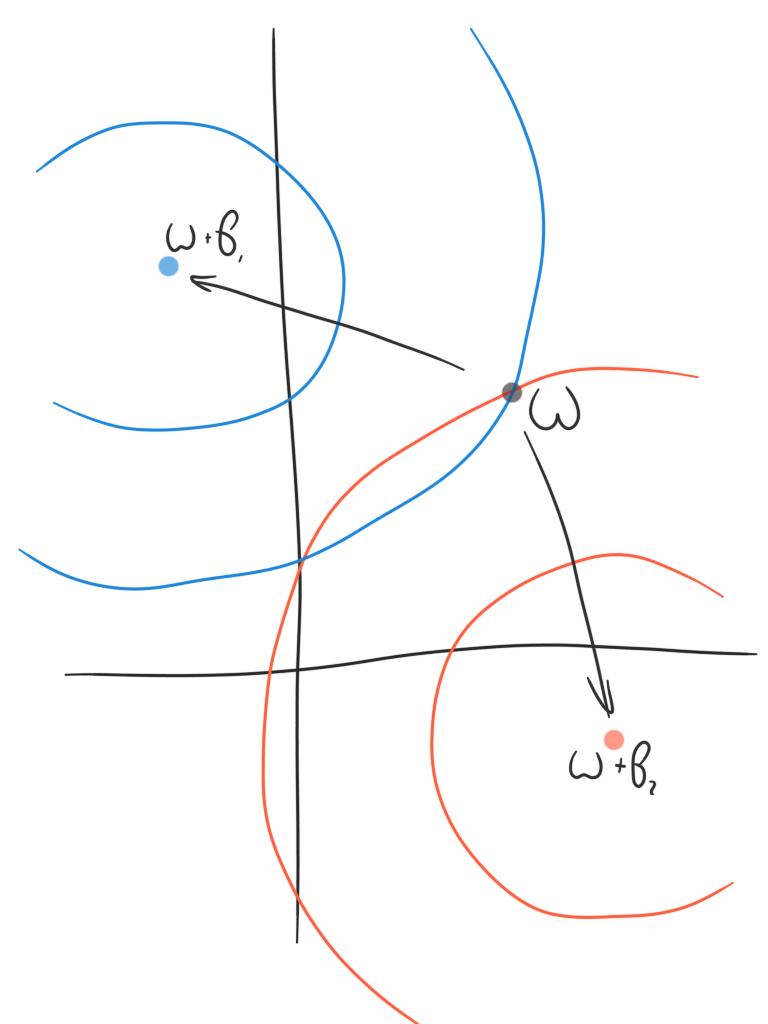
\includegraphics[scale=0.18]{pics/battaglini01.png}
		\end{center}
	\end{column}
	\begin{column}{0.5\textwidth}
		{\small
			\begin{itemize}
				\item Relative positions of bliss points and indifference curves are fixed; just the absolute location unknown.
			\end{itemize}
		}
	\end{column}
\end{columns}
\lyxframeend


\lyxframe{Idea}
\begin{columns}
	\begin{column}{0.5\textwidth}
		\begin{center}
			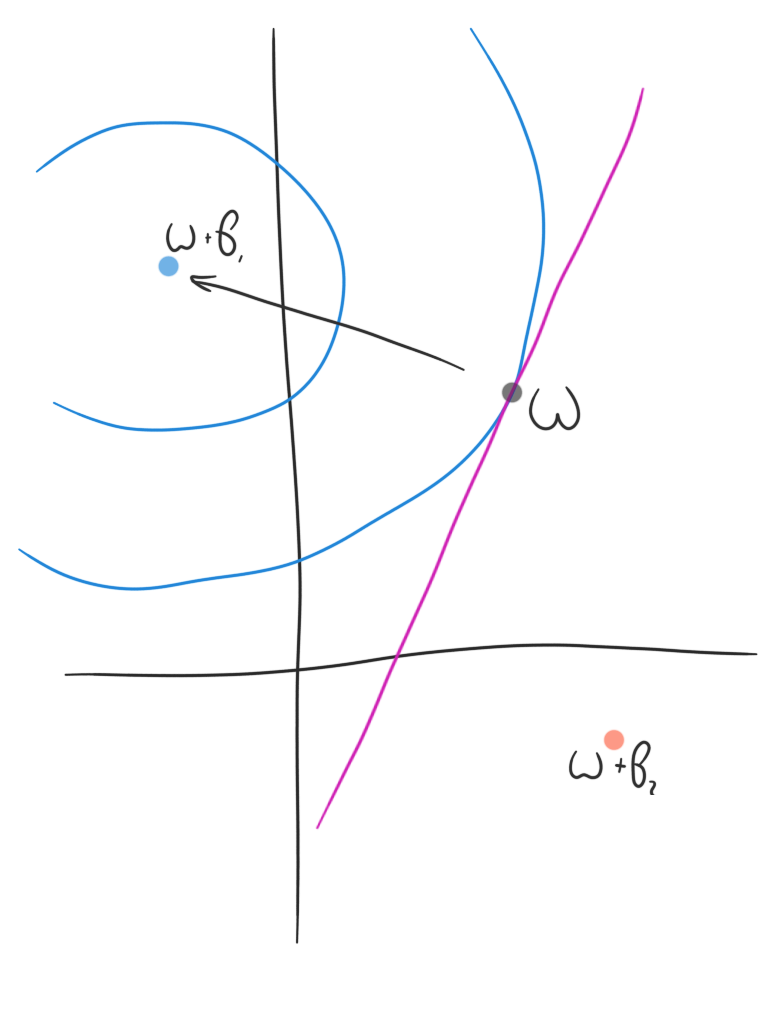
\includegraphics[scale=0.18]{pics/battaglini02.png}
		\end{center}
	\end{column}
	\begin{column}{0.5\textwidth}
		{\small
			\begin{itemize}
				\item Ask player $i$ to project the state on a line orthogonal to $b_i$ and report the result.
				\item Will report honestly.
			\end{itemize}
		}
	\end{column}
\end{columns}
\lyxframeend


\lyxframe{Idea}
\begin{columns}
	\begin{column}{0.5\textwidth}
		\begin{center}
			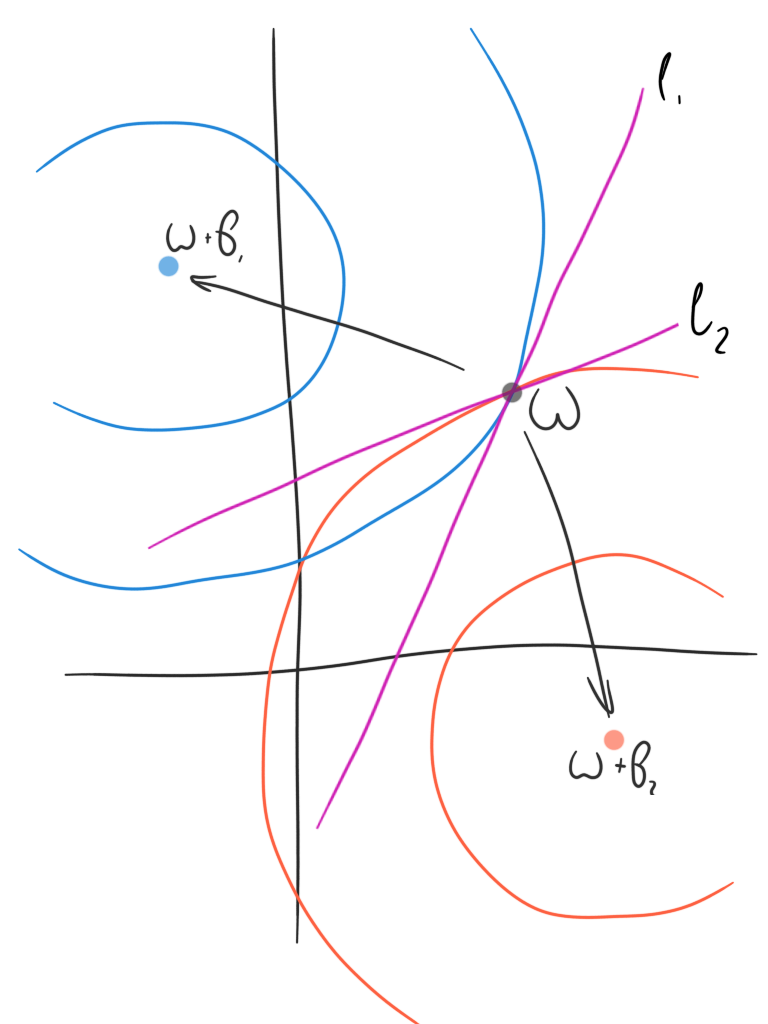
\includegraphics[scale=0.18]{pics/battaglini03.png}
		\end{center}
	\end{column}
	\begin{column}{0.5\textwidth}
		{\small
			\begin{itemize}
				\item With two players, can learn state perfectly this way.
				\item (As long as $b_i$ \structure{linearly independent}.)
				\item More generally, two players are enough to learn the state of any dimensionality $n$, since asking either player allows to learn $n-1$ dimensions of state.
				\item See Battaglini (2003) for $n$ dimensions and more general preferences.
			\end{itemize}
		}
	\end{column}
\end{columns}
\lyxframeend


\lyxframe{Equilibrium strategies}
\begin{columns}
	\begin{column}{0.5\textwidth}
		\begin{center}
			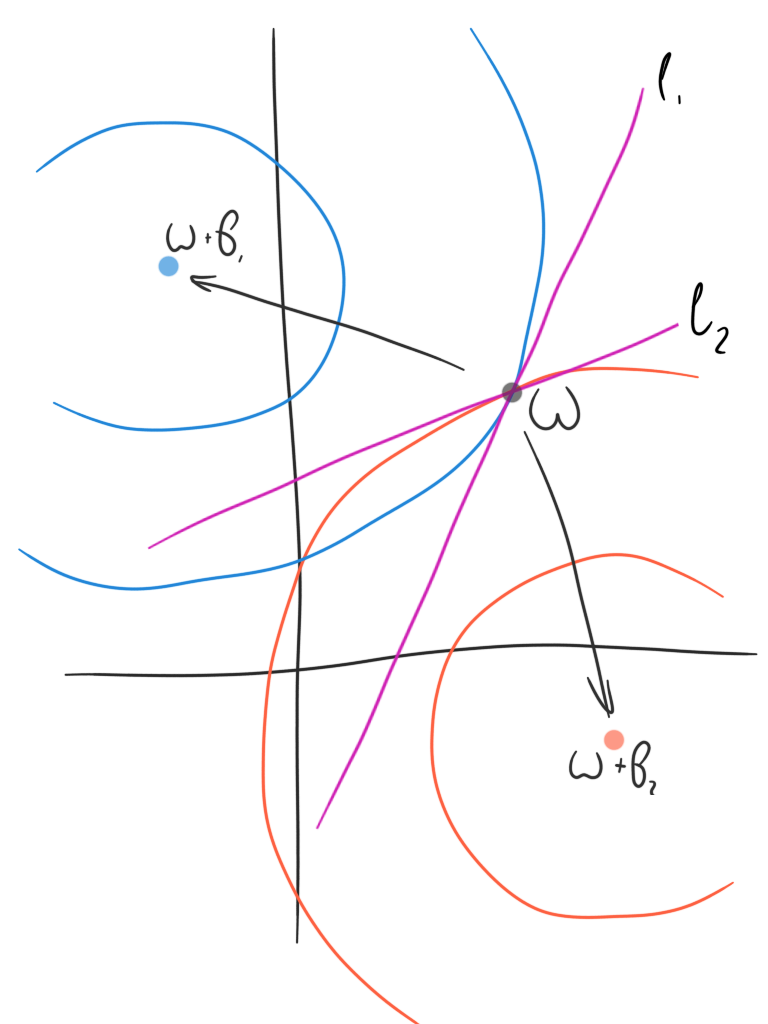
\includegraphics[scale=0.18]{pics/battaglini03.png}
		\end{center}
	\end{column}
	\begin{column}{0.5\textwidth}
		{\small
			\begin{itemize}
				\item Consider basis $(b_1,b_2)$. State $\omega$ has unique coordinates $(\omega_1^*,\omega_2^*)$ in this basis.
				\item Ask P1 to report $\omega_2^*$. This will determine the position of line $l_2$. I.e., P1 chooses where $l_2$ will intersect $l_1$ (which is fixed given report of P2).
				\item Then if P2 tells truth, it is optimal for P1 to report truth -- choose such $l_2$ which intersects $l_1$ at point to which $\omega+b_1$ is projected -- this point is the true $\omega$.
			\end{itemize}
		}
	\end{column}
\end{columns}
\lyxframeend


\lyxframe{Correlated information: Conclusion}
\begin{itemize}
	\item \structure{Correlated information} can be \alert{\textbf{very} easily exploited}; many ways to do so:
	\begin{itemize}
		\item If players' preferences conflict -- set them against each other (divide et impera);
		\item If players' preferences same -- force them to verify each other's reports.
	\end{itemize}
	\item Of course there are always issues that can arise:
	\begin{itemize}
		\item If players can communicate outside of the mechanism, collusion is a real threat.
		\item Cross-vefication may require making incredible or infeasible threats.
	\end{itemize}
\end{itemize}
\lyxframeend




\section{Lecture 6 \\ Dynamic Mechanism Design}

\lyxframe{Dynamic Problems}
\begin{itemize}
	\item Models considered so far were static: one report, one outcome.
	\begin{itemize}
		\item Although we hinted towards dynamic incentives when discussing interim vs ex post IC/IR constraints.
	\end{itemize}
	\item There are many dynamic problems in the real world:
	\begin{itemize}
		\item Dynamic pricing when buyers' tastes evolve (e.g. experience goods);
		\item Procurement from firms with changing costs;
		\item Design of tax and social security systems;
		\item Dynamic labor contracts
	\end{itemize}
	\item How to develop dynamic mechanisms? Will see today.
	\item This lecture mostly follows Bergemann and V�lim�ki (2019).
\end{itemize}
\lyxframeend


\lyxframe{Dynamic Problems}
\begin{itemize}
	\item First, what defines a dynamic problem? Why can it not be seen as a sequence of independent static problems? 
	\item The possible \structure{linkages} across periods include:
	\begin{enumerate}
		\item \alert{Information} -- future info evolves from (so depends on) past info and possibly past allocations.
		\item \alert{Preferences} -- usually evolve gradually. For our purposes, this is only relevant through serial correlation of information.
		\item \alert{Allocations} -- set of feasible allocations today may depend on past outcomes (example: sale of fixed number of items over many periods).
	\end{enumerate}
	\item The most important for our purposes is, of course, information.
\end{itemize}
\lyxframeend


\lyxframe{Dynamic Model}
\begin{itemize}
	\item \structure{Periods} $t \in \{0,2,...,T\}$; terminal time $T \leq \infty$; all players (incl. designer) have common \structure{discount} factor $\delta$.
	\item \structure{Players} $i \in \{1,2,...,N\}$ have evolving \structure{types} $\theta_{i,t} \in \Theta_i \subset \mathbb{R}$, indep. across $i$.
	\item Every period: \structure{allocation} $k_t \in K_t$ and \structure{payments} $p_t \in \mathbb{R}$.
	\item Players' \structure{utilities}: $u_i(k_t,p_t,\theta_t) = v_i(k_t,\theta_{i,t}) - p_{i,t}$.
	\item Common \structure{prior} $\theta_{i,0} \sim F_{i,0}$; \structure{types} are Markov processes: $$\theta_{i,t+1} \sim F_i(\theta_{i,t+1} | \theta_{i,t},k_t).$$
	\item Set of \structure{feasible} allocations evolves as $K_{t+1} = g(K_t,k_t)$.
\end{itemize}
\lyxframeend


\lyxframe{Evolving Types}
Possible interpretations of evolving types:
\begin{itemize}
	\item Exogenous evolution ($\theta_{t+1} \perp k$);
	\begin{itemize}
		\item Example: procuring goods over time from a firm with stochastically evolving costs $\theta_{i,t+1} = \gamma \theta_{i,t} + \varepsilon_{i,t+1}$.
	\end{itemize}
	\item Endogenous evolution (depending on $k_t$);
	\begin{itemize}
		\item Example: worker assigned to training by $k_t$ will improve their future productivity $\theta_{i,t+1}$.
	\end{itemize}
	\item Random arrival;
	\begin{itemize}
		\item Players can arrive at the mechanism at random times.
		\item Can model that by setting $\theta_{i,t} = 0$ whenever $i$ is not in the market/mechanism.
	\end{itemize}
\end{itemize}
\lyxframeend


\lyxframe{Dynamic Model: Assumptions}
To fix ideas, assume the following for today:
\begin{itemize}
	\item The designer can \structure{commit} to the whole future mechanism at $t=0$.
	\item All past reports and allocations are publicly observed.
	\item Player $i$ at time $t$ observes their type $\theta_{i,t}$ but not future types.
\end{itemize}
\lyxframeend


\lyxframe{Direct Mechanisms}
\begin{itemize}
	\item As usual, we have the revelation principle (Sugaya and Wolitzky, 2017).
	\item So can focus on mechanisms which ask players to report their types every period.
	\item Reporting strategies given by $\rho_i = \{r_{i,t}\}_{t=0}^T$, where $r_{i,t}: \Theta_i \times H_t \to \Theta_i$ and $H_t$ is the set of public histories $h_t = \{k_s,r_{i,s}\}_{s < t}$.
	\item A dynamic direct mechanism is $(\kappa,\pi) = \{k_t,p_t\}_{t=0}^T$, where $k_t: \Theta \times H_t \to K_t$ and $p_t: \Theta \times H_t \to \mathbb{R}^N$.
\end{itemize}
\lyxframeend


\lyxframe{Dynamic Implementation}
\begin{itemize}
	\item Looking for a truthful equilibrium in a direct mechanism.
	\item ``Equilibrium'' is a sketchy term in dynamic incomplete-info games.
	\begin{itemize}
		\item There is at least a dozen different equilibrium concepts and refinements in use.
		\item Main concern in general: off-equilibrium-path beliefs. What should a player believe after observing an event they considered impossible? Different answers can strongly affect the predicted outcome.
		\item Not a big problem in mechdesign.
	\end{itemize}
	\item Just look at standard \structure{Perfect Bayesian Equilibria}.
	\begin{itemize}
		\item Each player chooses report to maximize expected util, expecting others to report truthfully.
	\end{itemize}
\end{itemize}
\lyxframeend


\section{Efficient Dynamic Implementation}

\lyxframe{Efficient Allocation}
\begin{itemize}
	\item Suppose we want to implement the \structure{efficient allocation} $\kappa^*$.
	\item But what is $\kappa^*$ in a dynamic problem?
	$$ \kappa^* \in \arg \max_{\{k_t \in K_t\}_{t=0}^T} \mathbb{E} \left\{ \sum_{t=0}^T \delta^t \sum_{i=0}^N v_i(k_t,\theta_{i,t}) \right\}$$
	\item Today's allocation $k_t$ will affect tomorrow's types $\theta_{t+1}$ and set of alternatives $K_{t+1}$.
	\item Even finding the efficient allocation can in general be a difficult optimal control problem.
\end{itemize}
\lyxframeend


\lyxframe{Efficient Implementation}
\begin{itemize}
	\item Ok, suppose we found $\kappa^*$, what next?
	\item In static setting we used VCG aka the pivot mechanism: each player had to pay the externality they imposed on everyone else:
	$$ p_i(\theta) = -\sum_{j \neq i} v_j \left( k^*(\theta),\theta_j \right) + \sum_{j \neq i} v_j \left( k^*_{-i}(\theta_{-i}),\theta_j \right) $$
	\item The idea translates almost verbatim to the dynamics.
	\item Enter \structure{dynamic pivot mechanism}! (Bergemann and V�lim�ki, 2010)
\end{itemize}
\lyxframeend


\lyxframe{Dynamic Pivot Mechanism}
\begin{align*}
&\text{Flow social surplus}	& w(k_t,\theta_t)	&\equiv \sum_{i=0}^N v_i(k_t,\theta_{i,t}).
\\
&\text{Welfare}	& W(\theta_t,K_t)	&\equiv \max_{k_t \in K_t} \left\{ w(k_t,\theta_t) + \delta \mathbb{E} W(\theta_{t+1},K_{t+1}) \right\}.
\\
&\text{\footnotesize $i$'s marginal contribution}	& M_i(\theta_t,K_t)	&\equiv W(\theta_t,K_t) - W_{-i}(\theta_t,K_t)
\\
&\text{\footnotesize can be written recursively as}	& M_i(\theta_t,K_t)	&= m_i(\theta_t,K_t) + \delta \mathbb{E} M_i(\theta_t,K_t).
\\
&\text{Payments}	& p_{i,t}^*	&\equiv v_i(k^*_t,\theta_{i,t}) - m_i(\theta_t,K_t).
\end{align*}
\begin{itemize}
	\item The dynamic pivot mechanism is given by \structure{$\kappa = \kappa^*$} and \structure{$\rho = \{ p_{i,t}^* \}_{t=0}^T$}.
	\item Note that $i$ must pay his \structure{flow marginal contribution} rather than simply $w(k^*)-w(k^*_{-i})$.
	\item This is because $i$ by influencing today's allocation $k_t$, $i$ will also affect future types of other players and the set of available allocation -- have to account for that.
\end{itemize}
\lyxframeend


\section{Dynamic Revenue Maximization}

\lyxframe{}
\begin{itemize}
	\item 
\end{itemize}
\lyxframeend


\lyxframe{}
\begin{itemize}
	\item 
\end{itemize}
\lyxframeend


\lyxframe{}
\begin{itemize}
	\item 
\end{itemize}
\lyxframeend


\lyxframe{}
\begin{itemize}
	\item 
\end{itemize}
\lyxframeend


\lyxframe{}
\begin{itemize}
	\item 
\end{itemize}
\lyxframeend


\lyxframe{}
\begin{itemize}
	\item 
\end{itemize}
\lyxframeend


\end{document}